\documentclass{article}

\usepackage{amsmath, amssymb, bm}
\usepackage[a4paper, margin=1in]{geometry}
\usepackage{graphicx}

\title{State estimator}
\author{}
\date{}

\begin{document}
	
	\maketitle
	\section{Introduction}
	This document outlines the state estimator required for autonomous drone control. The primary objective is to estimate the state vector:
	
	\[
	\mathbf{x} =
	\begin{bmatrix}
		\mathbf{p} \\
		\mathbf{v} \\
		\mathbf{q} \\
		\mathbf{b}_g \\
		\mathbf{b}_a
	\end{bmatrix}
	\]
	
	The individual components of the state vector are defined as follows:
	
	\begin{itemize}
		\item $\mathbf{p} = [p_x, p_y, p_z]^\top$ is the position of the drone expressed in the world frame.
		
		\item $\mathbf{v} = [v_x, v_y, v_z]^\top$ is the linear velocity of the drone expressed in the world frame.
		
		\item $\mathbf{q} = [q_w, q_x, q_y, q_z]^\top$ is the unit quaternion describing the rotation from the drone body frame to the world frame, satisfying
		\[
		\|\mathbf{q}\| = 1.
		\]
		
		\item $\mathbf{b}_g = [b_{gx}, b_{gy}, b_{gz}]^\top$ is the gyroscope bias, representing a slowly varying offset in the measured angular velocity.
		
		\item $\mathbf{b}_a = [b_{ax}, b_{ay}, b_{az}]^\top$ is the accelerometer bias, representing a slowly varying offset in the measured specific force.
	\end{itemize}
	
	Thus, the nominal state vector consists of 16 elements ($3 + 3 + 4 + 3 + 3$).
	
	To estimate this state, we employ an Error-State Extended Kalman Filter (ES-EKF). The remainder of this document is organized as follows: we first lay out the theoretical foundation of the standard Kalman filter, extend it to the error-state formulation, and finally present the practical implementation details for our drone state estimator.
	
	\section{Standard Kalman Filter}
	
	The fundamental concept underlying the standard Kalman filter as a state estimator relies on two core steps:
	\begin{itemize}
		\item \textbf{Prediction:} Projecting the future state using the current state estimate and control inputs via a dynamic model.
		\item \textbf{Measurement update:} Fusing this predicted state with noisy sensor measurements.
	\end{itemize}
	A key strength of the Kalman filter is its ability to stochastically model the uncertainties associated with both the state propagation and the sensor readings. By evaluating these error covariances, the filter dynamically determines the optimal weighting—balancing model predictions against physical measurements to yield the best estimate.
	
	It is important to note that state estimation using a Kalman filter is a continuous, iterative process. At each discrete time step $k$, the filter propagates its internal belief forward using system dynamics (Prediction) and refines this belief at time step $k+1$ whenever new sensor data becomes available (Measurement Update). The \textit{a posteriori} output of time step $k$ serves directly as the initial condition for the prediction step at time step $k+1$, forming a closed feedback loop as illustrated in Figure~\ref{fig:my_figure}.
	
	\begin{figure}[htbp]
		\centering
		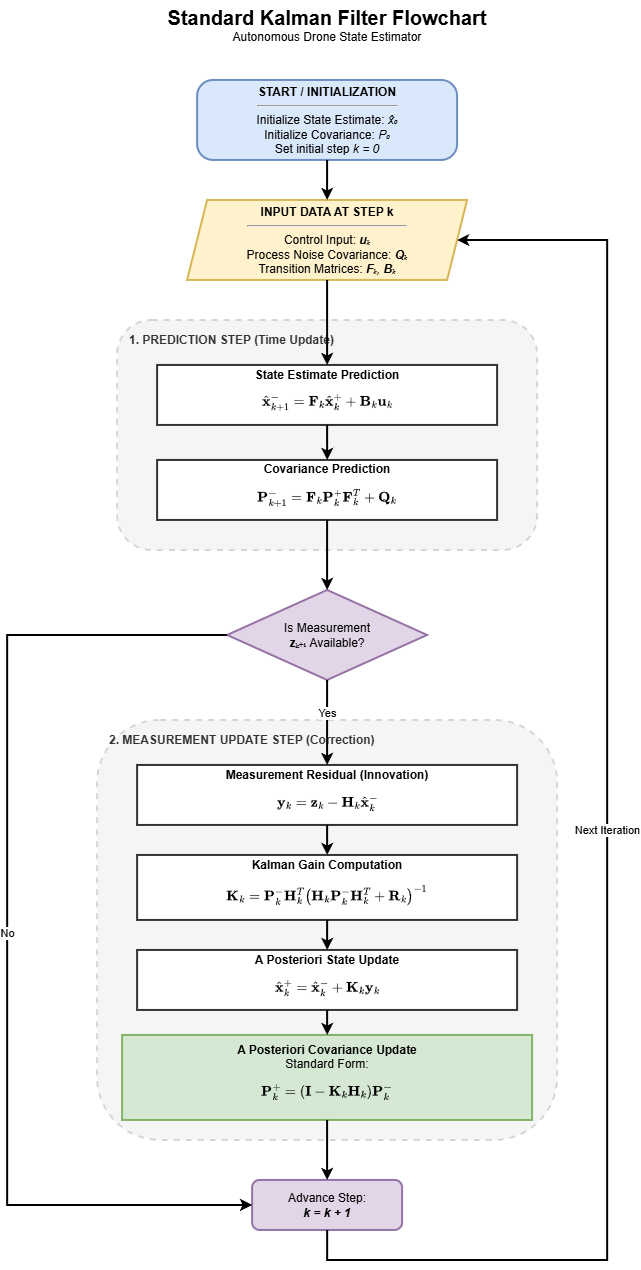
\includegraphics[width=0.8\textwidth]{flowchart.drawio.png}
		\caption{Visualization of different steps in a kalman filter}
		\label{fig:my_figure}
	\end{figure}
	
	
	
	\subsection{Prediction step}
	Assuming a discrete-time linear time-invariant (LTI) system, the state propagation step predicts the state at time step $k+1$ given the current state ($\mathbf{x}_{k}$) and some input ($\mathbf{u}_{k}$) at time step $k$:
	
	The \textbf{true state} evolves according to the physical dynamics subject to unobservable process noise $\mathbf{w}_{k} \sim \mathcal{N}(\mathbf{0}, \mathbf{Q})$:
	\begin{equation}
		\mathbf{x}_{k+1} = \mathbf{F} \mathbf{x}_{k} + \mathbf{B} \mathbf{u}_{k} + \mathbf{w}_{k}
		\label{eq:true_state_prop}
	\end{equation}
	
	Because process noise cannot be known in practice, the \textbf{predicted state estimate} is propagated by taking the conditional expectation ($\mathbb{E}[\mathbf{w}_{k}] = \mathbf{0}$):
	\begin{equation}
		\hat{\mathbf{x}}_{k+1}^- = \mathbf{F} \hat{\mathbf{x}}_{k}^+ + \mathbf{B} \mathbf{u}_{k}
		\label{eq:estimated_state_prop}
	\end{equation}
	
	Here, $\mathbf{F}$ denotes the state transition matrix, $\mathbf{B}$ is the control-input matrix, and $\mathbf{u}_{k}$ is the control vector at time step $k$.
	
	Several key observations follow from this formulation:
	\begin{itemize}
		\item We never have access to the true state $\mathbf{x}_{k}$; instead, we maintain an estimate, denoted by $\hat{\mathbf{x}}_{k}$.
		\item Rather than treating state and noise variables as deterministic vectors with scalar elements, we model them as \textbf{random vectors} whose elements are governed by probability distributions.
	\end{itemize}
	
	In the scalar case, a univariate probability distribution is characterized by its variance $\sigma^2$:
	\[
	\sigma^2 = \text{Var}(X) = \mathbb{E}\left[(X - \mu)^2\right]
	\]
	where $\mu = \mathbb{E}[X]$ is the mean (expected value) of the random variable $X$. 
	
	There is also the concept of covariance, which describes how two random variables vary together. For two random variables $X$ and $Y$, the covariance is defined as:
	\[
	\operatorname{Cov}(X,Y) = \mathbb{E}\left[(X-\mathbb{E}[X])(Y-\mathbb{E}[Y])\right].
	\]
	
	For example, suppose we independently sample values from two distributions $X$ and $Y$. If a sample from $X$ is larger than its mean, and this tends to coincide with a sample from $Y$ that is also larger than its mean, the two variables have positive covariance. Conversely, if a value of $X$ above its mean tends to coincide with a value of $Y$ below its mean, they have negative covariance. A covariance of zero means that there is no linear relationship between the two variables.
	
	Extending this concept to the Kalman filter, we are interested in the uncertainty of our state estimate. We define the estimation error as the difference between the true state and its estimate:
	\[
	\mathbf{e} = \mathbf{x} - \hat{\mathbf{x}}.
	\]
	
	The Kalman filter represents this error as a random variable with a probability distribution. We are particularly interested in its mean and covariance. Assuming the error has zero mean,
	\[
	\mathbb{E}[\mathbf{e}] = \mathbf{0},
	\]
	the covariance of the estimation error is defined as:
	\[
	\mathbf{P} = \mathbb{E}\left[\mathbf{e}\mathbf{e}^\top\right].
	\]
	
	Substituting the definition of the error gives:
	\[
	\boxed{
		\mathbf{P} = \mathbb{E}\left[(\mathbf{x}-\hat{\mathbf{x}})(\mathbf{x}-\hat{\mathbf{x}})^\top\right]
	}
	\]
	
	The outer product $\mathbf{e}\mathbf{e}^\top$ produces a matrix containing the variance of every state on the main diagonal and the covariance between every pair of states on the off-diagonals:
	\[
	\mathbf{P} = 
	\begin{bmatrix}
		\mathbb{E}[e_1^2] & \mathbb{E}[e_1 e_2] & \cdots & \mathbb{E}[e_1 e_n] \\
		\mathbb{E}[e_2 e_1] & \mathbb{E}[e_2^2] & \cdots & \mathbb{E}[e_2 e_n] \\
		\vdots & \vdots & \ddots & \vdots \\
		\mathbb{E}[e_n e_1] & \mathbb{E}[e_n e_2] & \cdots & \mathbb{E}[e_n^2]
	\end{bmatrix}.
	\]
	
	Therefore,
	\[
	P_{ii} = \operatorname{Var}(e_i)
	\]
	represents the variance of the error in state $i$, while
	\[
	P_{ij} = \operatorname{Cov}(e_i, e_j)
	\]
	represents the covariance between the errors of states $i$ and $j$.
	
	Thus, the covariance matrix $\mathbf{P}$ provides a description of the uncertainty of the state estimate: it tells the Kalman filter not only how uncertain each individual state is, but also how the uncertainties of different states are related to one another.
	
	Now that we know what the covariance matrix is we will discuss what happens with the covariance matrix when we predict the next step:
	\[
	\mathbf{e}_{k+1}^- = \mathbf{x}_{k+1} - \hat{\mathbf{x}}_{k+1}^-
	\]
	
	Substitution of equations \ref{eq:true_state_prop} and \ref{eq:estimated_state_prop} yields the dynamic propagation of the state error vector:
	\[
	\mathbf{e}_{k+1}^- = (\mathbf{F} \mathbf{x}_{k} + \mathbf{B} \mathbf{u}_{k} + \mathbf{w}_{k}) - (\mathbf{F} \hat{\mathbf{x}}_{k}^+ + \mathbf{B} \mathbf{u}_{k}) = \mathbf{F} (\mathbf{x}_{k} - \hat{\mathbf{x}}_{k}^+) + \mathbf{w}_{k} = \mathbf{F} \mathbf{e}_{k}^+ + \mathbf{w}_{k}
	\]
	
	By definition, the predicted error covariance matrix $\mathbf{P}_{k+1}^-$ is the expected value of the outer product of the prior error vector $\mathbf{e}_{k+1}^-$ with itself:
	\[
	\mathbf{P}_{k+1}^- = \mathbb{E} \left[ \mathbf{e}_{k+1}^- (\mathbf{e}_{k+1}^-)^T \right]
	\]
	
	Substituting the error propagation expression into the expectation gives:
	\begin{align*}
		\mathbf{P}_{k+1}^- &= \mathbb{E} \left[ (\mathbf{F} \mathbf{e}_{k}^+ + \mathbf{w}_{k})(\mathbf{F} \mathbf{e}_{k}^+ + \mathbf{w}_{k})^T \right] \\
		&= \mathbb{E} \left[ (\mathbf{F} \mathbf{e}_{k}^+ + \mathbf{w}_{k})((\mathbf{e}_{k}^+)^T \mathbf{F}^T + \mathbf{w}_{k}^T) \right] \\
		&= \mathbb{E} \left[ \mathbf{F} \mathbf{e}_{k}^+ (\mathbf{e}_{k}^+)^T \mathbf{F}^T + \mathbf{F} \mathbf{e}_{k}^+ \mathbf{w}_{k}^T + \mathbf{w}_{k} (\mathbf{e}_{k}^+)^T \mathbf{F}^T + \mathbf{w}_{k} \mathbf{w}_{k}^T \right]
	\end{align*}
	
	Since the state transition matrix $\mathbf{F}$ is deterministic, it can be factored out of the expectation operator. Applying linearity of expectation yields:
	\[
	\mathbf{P}_{k+1}^- = \mathbf{F} \mathbb{E}\left[\mathbf{e}_{k}^+ (\mathbf{e}_{k}^+)^T\right] \mathbf{F}^T + \mathbf{F} \mathbb{E}\left[\mathbf{e}_{k}^+ \mathbf{w}_{k}^T\right] + \mathbb{E}\left[\mathbf{w}_{k} (\mathbf{e}_{k}^+)^T\right] \mathbf{F}^T + \mathbb{E}\left[\mathbf{w}_{k} \mathbf{w}_{k}^T\right]
	\]
	
	Assuming that the process noise $\mathbf{w}_{k}$ is zero-mean and uncorrelated with the previous estimation error $\mathbf{e}_{k}^+$, the cross-terms vanish ($\mathbb{E}\left[\mathbf{e}_{k}^+ \mathbf{w}_{k}^T\right] = \mathbf{0}$). Recognizing $\mathbf{P}_{k}^+ = \mathbb{E}\left[\mathbf{e}_{k}^+ (\mathbf{e}_{k}^+)^T\right]$ and the process noise covariance $\mathbf{Q} = \mathbb{E}\left[\mathbf{w}_{k} \mathbf{w}_{k}^T\right]$, we arrive at the covariance prediction step equation:
	\begin{equation}
		\mathbf{P}_{k+1}^- = \mathbf{F} \mathbf{P}_{k}^+ \mathbf{F}^T + \mathbf{Q}
		\label{eq:covariance_propagation}
	\end{equation}
	
	In summary, the prediction step of the discrete-time linear Kalman filter propagates both the state estimate and its associated uncertainty forward from time step $k$ to $k+1$ using the system model before any new measurement is incorporated:
	\begin{enumerate}
		\item \textbf{True State Propagation} (\ref{eq:true_state_prop}): Models the unobservable physical dynamics of the system, perturbed by white process noise $\mathbf{w}_{k}$.
		\item \textbf{State Estimate Prediction} (\ref{eq:estimated_state_prop}): Projects our expected state forward using known control inputs $\mathbf{u}_{k}$ and state transition dynamics $\mathbf{F}$, assuming zero-mean process noise ($\mathbb{E}[\mathbf{w}_{k}] = \mathbf{0}$).
		\item \textbf{Covariance Prediction} (\ref{eq:covariance_propagation}): Quantifies how estimation uncertainty grows over time. The term $\mathbf{F} \mathbf{P}_{k}^+ \mathbf{F}^T$ maps current uncertainty through system dynamics, while $\mathbf{Q}$ accounts for additional uncertainty injected by unknown process disturbances.
	\end{enumerate}
	
	Together, these equations form the time-update phase of the Kalman filter, providing an a priori estimate $\hat{\mathbf{x}}_{k+1}^-$ alongside an updated measure of confidence $\mathbf{P}_{k+1}^-$ ready to be refined during the subsequent measurement update step.
	
	\section{Measurement Update Step}
	
	In the measurement update (or correction) step, the predicted state estimate $\hat{\mathbf{x}}_{k+1}^{-}$ (the \emph{a priori} estimate) is fused with a new observation vector $\mathbf{z}_{k+1}$ to compute the updated state estimate $\hat{\mathbf{x}}_{k+1}^{+}$ (the \emph{a posteriori} estimate).
	
	
	\noindent The updated state estimate $\hat{\mathbf{x}}_{k+1}^+$ is computed as:
	
	\begin{equation}
		\hat{\mathbf{x}}_{k+1}^+ = \hat{\mathbf{x}}_{k+1}^- + \mathbf{K} \left( \mathbf{z}_{k+1} - \mathbf{H} \hat{\mathbf{x}}_{k+1}^- \right)
		\label{eq:state_update}
	\end{equation}
	
	\noindent $\hat{\mathbf{x}}_{k+1}^-$ and $\hat{\mathbf{x}}_{k+1}^+$ are the \emph{a priori} and \emph{a posteriori} state estimates, respectively. We will go over the different elements of this equation in the upcoming subsections.
	
	
	\subsection{Measurement Residual and Innovation Covariance}
	
	The term $\left( \mathbf{z}_{k+1} - \mathbf{H} \hat{\mathbf{x}}_{k+1}^- \right)$ in Equation~\ref{eq:state_update} is defined as the \emph{measurement residual} (or \emph{innovation}):
	
	\begin{equation}
		\mathbf{y}_{k+1} = \mathbf{z}_{k+1} - \mathbf{H} \hat{\mathbf{x}}_{k+1}^-
		\label{eq:measurement_residual}
	\end{equation}
	
	Here, $\mathbf{z}_{k+1}$ is the observation vector containing raw sensor data acquired at step $k+1$. The observation matrix $\mathbf{H}$ maps the prior state estimate $\hat{\mathbf{x}}_{k+1}^-$ from the state space into the measurement space. 
	
	Applying $\mathbf{H}$ to $\hat{\mathbf{x}}_{k+1}^-$ yields a predicted measurement—representing what the sensors are expected to report based on the prior estimate. The difference between the actual measurement $\mathbf{z}_{k+1}$ and this prediction forms the residual $\mathbf{y}_{k+1}$, which quantifies the discrepancy between observation and prediction. As shown in Equation~\ref{eq:state_update}, this residual drives the state update, with its influence weighted by the Kalman gain $\mathbf{K}$.
	
	To compute the optimal Kalman gain, we must evaluate the uncertainty of this residual via its covariance matrix, denoted $\mathbf{S}_{k+1}$. Recalling the true measurement model,
	\begin{equation}
		\mathbf{z}_{k+1} = \mathbf{H} \mathbf{x}_{k+1} + \mathbf{v}_{k+1}
		\label{eq:true_measurement_model}
	\end{equation}
	where $\mathbf{x}_{k+1}$ is the true state and $\mathbf{v}_{k+1} \sim \mathcal{N}(\mathbf{0}, \mathbf{R}_{k+1})$ represents zero-mean measurement noise with covariance matrix $\mathbf{R}_{k+1}$. Substituting Equation~\ref{eq:true_measurement_model} into Equation~\ref{eq:measurement_residual} expresses the residual in terms of the prior estimation error $\mathbf{e}_{k+1}^- = \mathbf{x}_{k+1} - \hat{\mathbf{x}}_{k+1}^-$:
	
	\begin{align}
		\mathbf{y}_{k+1} &= \left(\mathbf{H} \mathbf{x}_{k+1} + \mathbf{v}_{k+1}\right) - \mathbf{H} \hat{\mathbf{x}}_{k+1}^- \nonumber \\
		&= \mathbf{H}\left(\mathbf{x}_{k+1} - \hat{\mathbf{x}}_{k+1}^-\right) + \mathbf{v}_{k+1} \nonumber \\
		&= \mathbf{H} \mathbf{e}_{k+1}^- + \mathbf{v}_{k+1}
		\label{eq:residual_error_form}
	\end{align}
	
	Assuming the prior estimation error $\mathbf{e}_{k+1}^-$ and the measurement noise $\mathbf{v}_{k+1}$ are uncorrelated with zero mean, the innovation covariance matrix $\mathbf{S}_{k+1} = \mathbb{E}\left[\mathbf{y}_{k+1} \mathbf{y}_{k+1}^T\right]$ is derived as:
	
	\begin{align}
		\mathbf{S}_{k+1} &= \mathbb{E}\left[ (\mathbf{H} \mathbf{e}_{k+1}^- + \mathbf{v}_{k+1}) (\mathbf{H} \mathbf{e}_{k+1}^- + \mathbf{v}_{k+1})^T \right] \nonumber \\
		&= \mathbb{E}\left[ \mathbf{H} \mathbf{e}_{k+1}^- (\mathbf{e}_{k+1}^-)^T \mathbf{H}^T + \mathbf{H} \mathbf{e}_{k+1}^- \mathbf{v}_{k+1}^T + \mathbf{v}_{k+1} (\mathbf{e}_{k+1}^-)^T \mathbf{H}^T + \mathbf{v}_{k+1} \mathbf{v}_{k+1}^T \right] \nonumber \\
		&= \mathbf{H} \mathbb{E}\left[ \mathbf{e}_{k+1}^- (\mathbf{e}_{k+1}^-)^T \right] \mathbf{H}^T + \mathbb{E}\left[ \mathbf{v}_{k+1} \mathbf{v}_{k+1}^T \right]
	\end{align}
	
	By substituting the prior error covariance matrix $\mathbf{P}_{k+1}^- = \mathbb{E}\left[ \mathbf{e}_{k+1}^- (\mathbf{e}_{k+1}^-)^T \right]$ and the measurement noise covariance matrix $\mathbf{R}_{k+1} = \mathbb{E}\left[ \mathbf{v}_{k+1} \mathbf{v}_{k+1}^T \right]$, we arrive at:
	
	\begin{equation}
		\mathbf{S}_{k+1} = \mathbf{H} \mathbf{P}_{k+1}^- \mathbf{H}^T + \mathbf{R}_{k+1}
		\label{eq:innovation_covariance}
	\end{equation}
	
	

	\subsubsection*{Example: Mapping State to Measurement space}
	
	Consider a system tracking 2D position and velocity, where the full state vector is defined as:
	\begin{equation*}
		\hat{\mathbf{x}}_{k+1} = 
		\begin{bmatrix} 
			p_x \\ p_y \\ v_x \\ v_y 
		\end{bmatrix}
	\end{equation*}
	
	Suppose our sensor setup consists solely of a GPS module capable of measuring position $(p_x, p_y)$, but not velocity. The observation vector $\mathbf{z}_{k+1}$ is therefore two-dimensional:
	\begin{equation*}
		\mathbf{z}_{k+1} = 
		\begin{bmatrix} 
			z_{p_x} \\ z_{p_y} 
		\end{bmatrix}
	\end{equation*}
	
	To isolate the position components from the full four-dimensional state, the observation matrix $\mathbf{H}$ is structured as:
	\begin{equation*}
		\mathbf{H} = 
		\begin{bmatrix} 
			1 & 0 & 0 & 0 \\ 
			0 & 1 & 0 & 0 
		\end{bmatrix}
	\end{equation*}
	
	Multiplying $\mathbf{H} \hat{\mathbf{x}}_{k+1}^-$ drops the unobserved velocity components and aligns the predicted state dimensions directly with the measurement vector:
	\begin{equation*}
		\mathbf{H} \hat{\mathbf{x}}_{k+1}^- = 
		\begin{bmatrix} 
			1 & 0 & 0 & 0 \\ 
			0 & 1 & 0 & 0 
		\end{bmatrix}
		\begin{bmatrix} 
			p_x \\ p_y \\ v_x \\ v_y 
		\end{bmatrix}
		= 
		\begin{bmatrix} 
			p_x \\ p_y 
		\end{bmatrix}
	\end{equation*}
	
	The residual vector $\mathbf{y}_{k+1}$ can then be evaluated directly in the measurement domain as $\begin{bmatrix} z_{p_x} - p_x \\ z_{p_y} - p_y \end{bmatrix}$.
	
	
	\subsection{Kalman Gain}
	
	Having computed the measurement residual $\mathbf{y}_{k+1}$ and its covariance matrix $\mathbf{S}_{k+1}$, we must update the \emph{a priori} state estimate $\hat{\mathbf{x}}_{k+1}^-$ to obtain the \emph{a posteriori} estimate $\hat{\mathbf{x}}_{k+1}^+$. The central challenge in state estimation is determining the optimal weighting between prediction and observation: balancing trust between the mathematical model and the incoming sensor data.
	
	This trade-off is governed by the \emph{Kalman gain} matrix $\mathbf{K}$:
	
	\begin{equation}
		\mathbf{K} = \mathbf{P}_{k+1}^{-} \mathbf{H}^T \mathbf{S}_{k+1}^{-1}
		\label{eq:kalman_gain}
	\end{equation}
	
	\noindent where:
	\begin{equation}
		\mathbf{S}_{k+1} = \mathbf{H} \mathbf{P}_{k+1}^{-} \mathbf{H}^T + \mathbf{R}_{k+1}
		\label{eq:innovation_covariance_ref}
	\end{equation}
	
	\noindent Here:
	\begin{itemize}
		\item $\mathbf{P}_{k+1}^-$ is the \emph{a priori} error covariance matrix, quantifying the expected uncertainty and correlations among errors in the predicted state estimate.
		\item $\mathbf{S}_{k+1}$ is the innovation (or residual) covariance matrix, representing the total uncertainty of the measurement residual, combining both projected state uncertainty and sensor noise.
		\item $\mathbf{R}_{k+1}$ is the measurement noise covariance matrix, representing the variance and noise characteristics of the physical sensors.
		\item $\mathbf{H}$ is the observation matrix mapping state space into measurement space.
	\end{itemize}
	
	\noindent By comparing projected state uncertainty against total innovation variance via $\mathbf{S}_{k+1}$, the Kalman gain dynamically scales the state update:
	\begin{itemize}
		\item If sensor noise is dominant ($\mathbf{R}_{k+1} \gg \mathbf{H} \mathbf{P}_{k+1}^- \mathbf{H}^T$), the innovation covariance becomes large ($\mathbf{S}_{k+1} \approx \mathbf{R}_{k+1}$), driving $\mathbf{K} \to \mathbf{0}$. The filter ignores noisy measurements and heavily weights the model prediction.
		\item If sensor noise is negligible ($\mathbf{R}_{k+1} \to \mathbf{0}$), the innovation uncertainty reduces to $\mathbf{S}_{k+1} \approx \mathbf{H} \mathbf{P}_{k+1}^- \mathbf{H}^T$. Consequently, $\mathbf{K}$ increases, forcing the updated state to rely predominantly on the incoming sensor measurement.
	\end{itemize}
	
	\noindent Selecting $\mathbf{K}$ according to Equation~\ref{eq:kalman_gain} is mathematically optimal: it minimizes the trace of the \emph{a posteriori} error covariance matrix $\mathbf{P}_{k+1}^+$, which corresponds to minimizing the mean-square error of the state estimate.	
	
	\section{Covariance Update}
	
	Having updated the state estimate $\hat{\mathbf{x}}_{k+1}^+$, we must update the \emph{a posteriori} error covariance matrix $\mathbf{P}_{k+1}^+$, which quantifies the residual uncertainty in our new estimate:
	
	\begin{equation}
		\mathbf{P}_{k+1}^+ = (\mathbf{I} - \mathbf{K} \mathbf{H}) \mathbf{P}_{k+1}^-
		\label{eq:cov_update}
	\end{equation}
	
	\noindent where $\mathbf{I}$ is the identity matrix of matching dimensions, $\mathbf{K}$ is the Kalman gain, $\mathbf{H}$ is the measurement matrix, and $\mathbf{P}_{k+1}^-$ is the \emph{a priori} error covariance matrix.
	
	For floating-point computer implementations, the \emph{Joseph form} formulation is often preferred to preserve symmetry and positive-definiteness:
	
	\begin{equation}
		\mathbf{P}_{k+1}^+ = (\mathbf{I} - \mathbf{K} \mathbf{H}) \mathbf{P}_{k+1}^- (\mathbf{I} - \mathbf{K} \mathbf{H})^T + \mathbf{K} \mathbf{R} \mathbf{K}^T
		\label{eq:cov_update_joseph}
	\end{equation}
	
	\subsection*{Variance Reduction via Gaussian Fusion}
	
	The core intuition behind this update lies in the properties of Gaussian probability distributions. Fusing two independent Gaussian distributions—the predicted state estimate $\mathcal{N}(\hat{\mathbf{x}}_{k+1}^-, \mathbf{P}_{k+1}^-)$ and the sensor measurement $\mathcal{N}(\mathbf{z}_{k+1}, \mathbf{R})$—yields a new Gaussian distribution $\mathcal{N}(\hat{\mathbf{x}}_{k+1}^+, \mathbf{P}_{k+1}^+)$ whose variance is strictly lower than either of the two input variances. 
	
	Because we are incorporating additional information into the system, our overall uncertainty decreases ($\mathbf{P}_{k+1}^+ \le \mathbf{P}_{k+1}^-$), sharpening the state estimate at each measurement step.
	
	\section{Kalman filter: practical example}
	Now that we have covered the underlying theory of the filter, let us work out a concrete 2D tracking example. Consider a vehicle moving in a two-dimensional plane ($x\text{--}y$). The vehicle is equipped with two sensors:
	\begin{itemize}
		\item A \textbf{GPS receiver} providing absolute position measurements $(p_x, p_y)$.
		\item An \textbf{accelerometer} measuring linear accelerations $(a_x, a_y)$ along the movement axes.
	\end{itemize}
	
	Our objective is to estimate the state vector $\mathbf{x} \in \mathbb{R}^4$, consisting of 2D position and velocity:
	\begin{equation}
		\mathbf{x}_k = 
		\begin{bmatrix}
			p_x \\
			p_y \\
			v_x \\
			v_y
		\end{bmatrix}
	\end{equation}
	
	In an ideal, noise-free environment, an initial state along with accelerometer readings would suffice to reconstruct the trajectory using basic kinematic integration:
	\begin{align*}
		\mathbf{v}(t) &= \mathbf{v}_0 + \int_{0}^{t} \mathbf{a}(\tau) \, d\tau \\
		\mathbf{p}(t) &= \mathbf{p}_0 + \int_{0}^{t} \mathbf{v}(\tau) \, d\tau
	\end{align*}
	
	In practice, however, raw accelerometer measurements suffer from noise and biases. Integrating noisy measurements over time causes numerical integration errors to accumulate, leading to severe \textit{position drift}. To eliminate this drift, we fuse the high-rate IMU/accelerometer data with absolute GPS position updates inside a Kalman filter framework. 
	
	Specifically, accelerometer measurements serve as the control input $\mathbf{u}_k$ during the prediction step, while GPS observations form the measurement vector $\mathbf{z}_k$ during the correction step.
	
	\subsection{System Modeling and State Propagation}
	
	Assuming a constant time step $\Delta t$, continuous kinematic integration discretized via Taylor expansion yields:
	\begin{align*}
		p_{x, k+1} &= p_{x, k} + v_{x, k} \Delta t + \frac{1}{2} a_{x, k} \Delta t^2 \\
		v_{x, k+1} &= v_{x, k} + a_{x, k} \Delta t
	\end{align*}
	
	We express this discrete linear system in standard state-space matrix notation:
	\begin{equation}
		\mathbf{x}_{k+1} = \mathbf{F} \mathbf{x}_k + \mathbf{B} \mathbf{u}_k + \mathbf{w}_k
	\end{equation}
	
	where the control input vector is $\mathbf{u}_k = [a_{x, k}, a_{y, k}]^\top$. The state transition matrix $\mathbf{F}$ and control-input matrix $\mathbf{B}$ are defined as:
	\begin{equation}
		\mathbf{F} = 
		\begin{bmatrix}
			1 & 0 & \Delta t & 0 \\
			0 & 1 & 0 & \Delta t \\
			0 & 0 & 1 & 0 \\
			0 & 0 & 0 & 1
		\end{bmatrix}, \quad
		\mathbf{B} = 
		\begin{bmatrix}
			\frac{1}{2}\Delta t^2 & 0 \\
			0 & \frac{1}{2}\Delta t^2 \\
			\Delta t & 0 \\
			0 & \Delta t
		\end{bmatrix}
	\end{equation}
	
	\subsection{Process Noise Covariance ($\mathbf{Q}$)}
	
	By definition, the process noise covariance matrix represents the expected outer product of the state noise vector $\mathbf{w}_k$ with itself:
	\begin{equation}
		\mathbf{Q} = \mathbb{E}\left[\mathbf{w}_k \mathbf{w}_k^\top\right]
	\end{equation}
	
	To compute $\mathbf{Q}$ in practice, we must trace where this state noise originates physically. In our system, the accelerometer readings act as control inputs $\mathbf{u}_k$. However, the physical sensors are subject to zero-mean Gaussian white noise $\mathbf{n}_a = [n_{ax}, n_{ay}]^\top$ with known variance $\sigma_a^2$:
	\begin{equation}
		\mathbf{u}_{\text{measured}} = \mathbf{u}_{\text{true}} + \mathbf{n}_a, \quad \text{where } \mathbf{n}_a \sim \mathcal{N}\left(\mathbf{0}, \mathbf{Q}_u\right)
	\end{equation}
	
	The sensor noise covariance matrix $\mathbf{Q}_u \in \mathbb{R}^{2 \times 2}$ is defined as:
	\begin{equation}
		\mathbf{Q}_u = \mathbb{E}\left[\mathbf{n}_a \mathbf{n}_a^\top\right] = 
		\begin{bmatrix}
			\sigma_a^2 & 0 \\
			0 & \sigma_a^2
		\end{bmatrix} = \sigma_a^2 \mathbf{I}_{2 \times 2}
	\end{equation}
	
	Substituting the noisy measurement $\mathbf{u}_{\text{measured}}$ into the system propagation equation reveals how sensor noise enters the state space:
	\begin{equation}
		\mathbf{x}_{k+1} = \mathbf{F}\mathbf{x}_k + \mathbf{B}(\mathbf{u}_{\text{true}} + \mathbf{n}_a) = \underbrace{\mathbf{F}\mathbf{x}_k + \mathbf{B}\mathbf{u}_{\text{true}}}_{\text{True Motion}} + \underbrace{\mathbf{B}\mathbf{n}_a}_{\text{State Noise } \mathbf{w}_k}
	\end{equation}
	
	Equating the noise term yields $\mathbf{w}_k = \mathbf{B}\mathbf{n}_a$. Substituting this back into the expectation definition gives:
	\begin{align}
		\mathbf{Q} &= \mathbb{E}\left[(\mathbf{B}\mathbf{n}_a)(\mathbf{B}\mathbf{n}_a)^\top\right] \nonumber \\
		&= \mathbb{E}\left[\mathbf{B}\mathbf{n}_a \mathbf{n}_a^\top \mathbf{B}^\top\right] \nonumber \\
		&= \mathbf{B} \, \mathbb{E}\left[\mathbf{n}_a \mathbf{n}_a^\top\right] \mathbf{B}^\top \nonumber \\
		&= \mathbf{B} \mathbf{Q}_u \mathbf{B}^\top = \sigma_a^2 \mathbf{B}\mathbf{B}^\top
	\end{align}
	
	Finally, evaluating the matrix product $\mathbf{B}\mathbf{B}^\top$ yields the explicit $4 \times 4$ process noise matrix $\mathbf{Q}$:
	\begin{equation}
		\mathbf{Q} = \sigma_a^2
		\begin{bmatrix}
			\frac{1}{4}\Delta t^4 & 0 & \frac{1}{2}\Delta t^3 & 0 \\
			0 & \frac{1}{4}\Delta t^4 & 0 & \frac{1}{2}\Delta t^3 \\
			\frac{1}{2}\Delta t^3 & 0 & \Delta t^2 & 0 \\
			0 & \frac{1}{2}\Delta t^3 & 0 & \Delta t^2
		\end{bmatrix}
	\end{equation}

	
	\subsection{Measurement Model ($\mathbf{H}$) and Measurement Noise ($\mathbf{R}$)}
	
	The GPS module directly measures position $(p_x, p_y)$, yielding a two-dimensional measurement vector $\mathbf{z}_k \in \mathbb{R}^2$:
	\begin{equation}
		\mathbf{z}_k = 
		\begin{bmatrix}
			z_{p_x} \\
			z_{p_y}
		\end{bmatrix}
	\end{equation}
	
	The measurement matrix $\mathbf{H}$ extracts the position components from the 4D state vector:
	\begin{equation}
		\mathbf{H} = 
		\begin{bmatrix}
			1 & 0 & 0 & 0 \\
			0 & 1 & 0 & 0
		\end{bmatrix}
	\end{equation}
	
	Assuming independent GPS measurement errors along the $x$ and $y$ axes with variance $\sigma_{\text{GPS}}^2$ (e.g., $\sigma_{\text{GPS}}^2 = 2.0 \text{ m}^2$), the measurement noise covariance matrix $\mathbf{R} \in \mathbb{R}^{2 \times 2}$ is given by:
	\begin{equation}
		\mathbf{R} = 
		\begin{bmatrix}
			\sigma_{\text{GPS}}^2 & 0 \\
			0 & \sigma_{\text{GPS}}^2
		\end{bmatrix}
	\end{equation}
	
	\subsection{Filter Initialization}
	
	Before running the predictive loop, we initialize the state vector $\hat{\mathbf{x}}_0^+$ and state covariance matrix $\mathbf{P}_0^+$. 
	
	If the initial position is obtained from the first GPS fix and the initial velocity is assumed to be zero, the state vector is initialized as:
	\begin{equation}
		\hat{\mathbf{x}}_0^+ = 
		\begin{bmatrix}
			z_{p_x, 0} \\
			z_{p_y, 0} \\
			0 \\
			0
		\end{bmatrix}
	\end{equation}
	
	The initial covariance matrix $\mathbf{P}_0^+$ represents our confidence in these starting values. Position uncertainty is tied directly to GPS accuracy ($\sigma_{\text{GPS}}^2$), while velocity uncertainty is set to a higher variance $\sigma_{v,0}^2$ to reflect initial guessing:
	\begin{equation}
		\mathbf{P}_0^+ = 
		\begin{bmatrix}
			\sigma_{\text{GPS}}^2 & 0 & 0 & 0 \\
			0 & \sigma_{\text{GPS}}^2 & 0 & 0 \\
			0 & 0 & \sigma_{v,0}^2 & 0 \\
			0 & 0 & 0 & \sigma_{v,0}^2
		\end{bmatrix}
	\end{equation}
	
	With $\mathbf{F}$, $\mathbf{B}$, $\mathbf{Q}$, $\mathbf{H}$, $\mathbf{R}$, $\hat{\mathbf{x}}_0^+$, and $\mathbf{P}_0^+$ fully specified, the filter executes sequentially across discrete time steps via the prediction and update equations derived in Sections 2 and 3.
	
	\section{Error-State Kalman Filter}
	
	In the previous section, the standard linear Kalman filter was introduced under the assumption of linear system dynamics and measurement models. However, physical systems encountered in engineering practice are frequently non-linear, evolving according to:
	
	\begin{equation}
		\mathbf{x}_{k+1} = f(\mathbf{x}_k, \mathbf{u}_k) + \mathbf{w}_k
	\end{equation}
	
	where $f(\cdot)$ represents the non-linear state transition function, $\mathbf{u}_k$ denotes the control input, and $\mathbf{w}_k \sim \mathcal{N}(\mathbf{0}, \mathbf{Q}_k)$ is additive, zero-mean Gaussian process noise. Similarly, measurements are modeled as:
	
	\begin{equation}
		\mathbf{z}_k = h(\mathbf{x}_k) + \mathbf{v}_k
	\end{equation}
	
	where $h(\cdot)$ is the non-linear measurement function and $\mathbf{v}_k \sim \mathcal{N}(\mathbf{0}, \mathbf{R}_k)$ represents additive, zero-mean Gaussian measurement noise.
	
	To handle non-linear functions, the Error-State Kalman Filter (ESKF) decouples the true state $\mathbf{x}$ into a large-signal \textbf{nominal state} $\hat{\mathbf{x}}$ and a small \textbf{error state} $\delta\mathbf{x}$:
	
	\begin{equation}
		\mathbf{x} = \hat{\mathbf{x}} + \delta\mathbf{x}
	\end{equation}
	
	The ESKF operates recursively through the following four-step loop:
	\begin{enumerate}
		\item \textbf{Nominal state propagation:} Integrate the non-linear system dynamics to propagate the nominal state forward in time, assuming zero noise.
		\item \textbf{Residual computation:} Make a measurement and compare it with the expected measurement based on the propagated state using the non-linear measurment function $h$ too compute the residual $\mathbf{y}$.
		\item \textbf{Kalman gain computation:} Compute the Kalman gain $\mathbf{K}$
		\item \textbf{Error state estimation:} Using the Kalman gian and the residual, compute the new error state $\delta\hat{\mathbf{x}}_{k+1}$.
		\item \textbf{State injection (correction):} Combine the estimated error state with the nominal state to update the true nominal state estimate, and update the error covariance matrix.
		\item \textbf{Error covariance update:} Now we have fused the predicted and measured value we need too update the uncertainty of the error estimate.
		\item \textbf{Error Reset:} Reset the expected error state to zero for the next filter iteration.
	\end{enumerate}
	
	\subsection{Nominal State Propagation}
	
	Since the non-linear dynamics function $f(\cdot)$ is known, the nominal state can be propagated forward in time as:
	
	\begin{equation}
		\hat{\mathbf{x}}_{k+1}^- = f(\hat{\mathbf{x}}_k^+, \mathbf{u}_k)
	\end{equation}
	
	\subsection{Residual computation}
	
	Too compute the residual we compare an actual measurement $\mathbf{z}_{k+1}$ to the expected measurement $\hat{\mathbf{z}}_{k+1}$. We can derive the expected measurement from the propagated state and the non-linear measurement function $h$:
	
	\begin{equation*}
		\hat{\mathbf{z}}_{k+1} = h(\hat{\mathbf{x}}_{k+1}^-, \mathbf{u}_k)
	\end{equation*}
	
	The residual is defined as the difference between these two quantities:
	\begin{equation*}
		\mathbf{y}_{k+1} = \mathbf{z}_{k+1} - \hat{\mathbf{z}}_{k+1}
	\end{equation*}
	
	\subsection{Kalman gain computation}
	Now that we have obtained the residual $\mathbf{y}_{k+1}$, we need too know how "much" of it we'll use too update the state. If we trust the measurement more then the propagated state we will use quite a bit of it. In case we don't we will use less of it. This is exactly what the Kalman gain $\mathbf{K}$ will allow us too do. In order to do so we need too know the uncertainty of the propagated error state $\delta\mathbf{x}$ which we'll denote with the covariance matrix $\mathbf{P}_{k+1}^-$. Next we need too know the uncertainty of the residual $\mathbf{y}_{k+1}$ which we'll denote with the innovation covariance matrix $\mathbf{S}_{k+1}^-$, the Kalman gain can then be computed using the following expression:
	
	\begin{equation*}
		\mathbf{K} = \mathbf{P}_{k+1}^- \mathbf{H}_{k+1}^T \mathbf{S}_{k+1}^{-1}
	\end{equation*}
	
	Please note $\mathbf{H}_{k+1}$ is the Jacobian matrix of the measurement function $h$. The presence of this term will become more clear in the upcoming sections.
	
	\subsubsection{The error state covariance matrix $\mathbf{P}$}
	
	Although the estimated error vector $\delta\mathbf{x}_k$ is reset to zero after each injection step, its associated covariance matrix $\mathbf{P}_k$ continues to grow during prediction due to process noise.
	
	To derive the propagation of the error state, we expand the non-linear process model $f(\mathbf{x}_k, \mathbf{u}_k)$ around the nominal state $\hat{\mathbf{x}}_k^+$ using a first-order Taylor series approximation:
	
	\begin{align}
		\mathbf{x}_{k+1} &= f(\mathbf{x}_k, \mathbf{u}_k) + \mathbf{w}_k \nonumber \\
		\hat{\mathbf{x}}_{k+1}^- + \delta\mathbf{x}_{k+1} &= f(\hat{\mathbf{x}}_k^+ + \delta\mathbf{x}_k, \mathbf{u}_k) + \mathbf{w}_k \nonumber \\
		&\approx f(\hat{\mathbf{x}}_k^+, \mathbf{u}_k) + \left. \frac{\partial f}{\partial \mathbf{x}} \right|_{\hat{\mathbf{x}}_k^+, \mathbf{u}_k} \delta\mathbf{x}_k + \mathbf{w}_k \\
		&\approx \hat{\mathbf{x}}_{k+1}^- + \mathbf{F}_k \delta\mathbf{x}_k + \mathbf{w}_k
	\end{align}
	
	Subtracting the nominal state propagation $\hat{\mathbf{x}}_{k+1}^- = f(\hat{\mathbf{x}}_k^+, \mathbf{u}_k)$ yields the linearized error dynamics:
	
	\begin{equation}
		\delta\mathbf{x}_{k+1} \approx \mathbf{F}_k \delta\mathbf{x}_k + \mathbf{w}_k
	\end{equation}
	
	where $\mathbf{F}_k = \left. \frac{\partial f}{\partial \mathbf{x}} \right|_{\hat{\mathbf{x}}_k^+, \mathbf{u}_k}$ is the error transition Jacobian matrix evaluated at the current nominal estimate.
	
	For standard vector spaces with additive state composition ($\mathbf{x} = \hat{\mathbf{x}} + \boldsymbol{\delta\mathbf{x}}$), applying the chain rule yields:
	
	\begin{equation*}
		\frac{\partial f(\mathbf{x})}{\partial \boldsymbol{\delta\mathbf{x}}} = \frac{\partial f(\mathbf{x})}{\partial \mathbf{x}} \cdot \frac{\partial \mathbf{x}}{\partial \boldsymbol{\delta\mathbf{x}}} = \frac{\partial f(\mathbf{x})}{\partial \mathbf{x}} \cdot \frac{\partial (\hat{\mathbf{x}} + \boldsymbol{\delta\mathbf{x}})}{\partial \boldsymbol{\delta\mathbf{x}}} = \frac{\partial f(\mathbf{x})}{\partial \mathbf{x}} \mathbf{I}
	\end{equation*}
	
	This allows the state transition matrix to be expressed equivalently as:
	
	\begin{equation*}
		\mathbf{F}_k = \left. \frac{\partial f}{\partial \mathbf{x}} \right|_{\hat{\mathbf{x}}_k^+, \mathbf{u}_k} = \left. \frac{\partial f}{\partial \boldsymbol{\delta\mathbf{x}}} \right|_{\boldsymbol{\delta\mathbf{x}} = \mathbf{0}, \mathbf{u}_k}
	\end{equation*}
	
	Throughout this work, we adopt the latter formulation (differentiating directly with respect to $\boldsymbol{\delta\mathbf{x}}$). While identical in vector spaces, evaluating derivatives directly with respect to the local error state naturally generalizes to non-linear manifolds (e.g., $SO(3)$), where state composition is non-additive ($\mathbf{x} = \hat{\mathbf{x}} \oplus \boldsymbol{\delta\mathbf{x}}$).
	
	The prior error covariance is then propagated forward in time:
	
	\begin{align}
		\mathbf{P}_{k+1}^- &= \mathbb{E}\left[ \delta\mathbf{x}_{k+1} \delta\mathbf{x}_{k+1}^T \right] \nonumber \\
		&= \mathbb{E}\left[ (\mathbf{F}_k \delta\mathbf{x}_k + \mathbf{w}_k)(\mathbf{F}_k \delta\mathbf{x}_k + \mathbf{w}_k)^T \right] \nonumber \\
		&= \mathbf{F}_k \mathbf{P}_k^+ \mathbf{F}_k^T + \mathbf{Q}_k
	\end{align}
	
	The key advantage of this formulation is that the predicted mean error $\delta\mathbf{x}_{k+1}$ does not need to be explicitly propagated. Because the error state is assumed to be zero-mean, its expectation under the linearized dynamics remains zero:
	
	\begin{equation}
		\mathbb{E}[\delta\mathbf{x}_{k+1}] = \mathbb{E}[\mathbf{F}_k \delta\mathbf{x}_k + \mathbf{w}_k] = \mathbf{F}_k \mathbb{E}[\delta\mathbf{x}_k] + \mathbb{E}[\mathbf{w}_k] = \mathbf{0}
	\end{equation}
	
	Consequently, the propagation step focuses entirely on tracking how the error covariance—the uncertainty and cross-correlations—evolves through the system dynamics.
	
	\subsubsection{The residual covariance matrix $\mathbf{S}$}
	
	When a sensor observation arrives, the measurement residual (or innovation) $\mathbf{y}_{k+1}$ measures the discrepancy between the physical observation $\mathbf{z}_{k+1}$ and the expected observation $\hat{\mathbf{z}}_{k+1}$:
	
	\begin{equation}
		\mathbf{y}_{k+1} = \mathbf{z}_{k+1} - \hat{\mathbf{z}}_{k+1}
	\end{equation}
	
	The real physical measurement is modeled via the non-linear measurement function $h(\cdot)$ perturbed by zero-mean measurement noise $\mathbf{v}_{k+1} \sim \mathcal{N}(\mathbf{0}, \mathbf{R}_{k+1})$:
	
	\begin{equation}
		\mathbf{z}_{k+1} = h(\mathbf{x}_{k+1}) + \mathbf{v}_{k+1}
	\end{equation}
	
	Similarly, the predicted measurement $\hat{\mathbf{z}}_{k+1}$ is computed by passing the propagated nominal state $\hat{\mathbf{x}}_{k+1}^-$ through the same non-linear mapping:
	
	\begin{equation}
		\hat{\mathbf{z}}_{k+1} = h(\hat{\mathbf{x}}_{k+1}^-)
	\end{equation}
	
	Direct substitution yields the actionable form of the measurement residual:
	
	\begin{equation}
		\mathbf{y}_{k+1} = \mathbf{z}_{k+1} - h(\hat{\mathbf{x}}_{k+1}^-)
	\end{equation}
	
	To compute the optimal Kalman gain, the uncertainty associated with this residual must be determined. Expressing the true state as $\mathbf{x}_{k+1} = \hat{\mathbf{x}}_{k+1}^- + \delta\mathbf{x}_{k+1}$ and expanding $h(\cdot)$ using a first-order Taylor series around the propagated nominal state gives:
	
	\begin{align}
		\mathbf{z}_{k+1} &= h(\hat{\mathbf{x}}_{k+1}^- + \delta\mathbf{x}_{k+1}) + \mathbf{v}_{k+1} \nonumber \\
		&\approx h(\hat{\mathbf{x}}_{k+1}^-) + \left. \frac{\partial h}{\partial \mathbf{x}} \right|_{\hat{\mathbf{x}}_{k+1}^-} \delta\mathbf{x}_{k+1} + \mathbf{v}_{k+1} \nonumber \\
		&= h(\hat{\mathbf{x}}_{k+1}^-) + \mathbf{H}_{k+1} \delta\mathbf{x}_{k+1} + \mathbf{v}_{k+1}
	\end{align}
	
	where $\mathbf{H}_{k+1} = \left. \frac{\partial h}{\partial \mathbf{x}} \right|_{\hat{\mathbf{x}}_{k+1}^-}$ is the measurement Jacobian matrix evaluated at the propagated nominal state. Substituting this linearized approximation into the residual expression yields:
	
	\begin{equation}
		\mathbf{y}_{k+1} \approx \mathbf{H}_{k+1} \delta\mathbf{x}_{k+1} + \mathbf{v}_{k+1}
	\end{equation}
	
	The residual uncertainty (innovation covariance $\mathbf{S}_{k+1}$) is computed as:
	
	\begin{align}
		\mathbf{S}_{k+1} &= \mathbb{E}\left[ \mathbf{y}_{k+1} \mathbf{y}_{k+1}^T \right] \nonumber \\
		&= \mathbb{E}\left[ (\mathbf{H}_{k+1} \delta\mathbf{x}_{k+1} + \mathbf{v}_{k+1})(\mathbf{H}_{k+1} \delta\mathbf{x}_{k+1} + \mathbf{v}_{k+1})^T \right] \nonumber \\
		&= \mathbf{H}_{k+1} \mathbf{P}_{k+1}^- \mathbf{H}_{k+1}^T + \mathbf{R}_{k+1}
	\end{align}
	

	\subsection{Error state estimation}
	
	Now that we have computed the residual $\mathbf{y}_{k+1}$ and the Kalman gain $\mathbf{K}$ we can estimate the error:
	
	\begin{equation}
		\delta\hat{\mathbf{x}}_{k+1} = \mathbf{K} \mathbf{y}_{k+1}
	\end{equation}
	
	As discussed previously, the Kalman gain provides the optimal weighting between the measured and predicted values to minimize the trace of the error state covariance matrix, thereby yielding the minimum-variance estimate.
	
	
	\subsection{State Injection}
	
	After estimating the error state $\delta\hat{\mathbf{x}}_{k+1}$ via the Kalman gain, it is injected into the propagated nominal state estimate to yield the updated posterior nominal state $\hat{\mathbf{x}}_{k+1}^+$ using vector addition:
	
	\begin{equation}
		\hat{\mathbf{x}}_{k+1}^+ = \hat{\mathbf{x}}_{k+1}^- + \delta\hat{\mathbf{x}}_{k+1}
	\end{equation}
	
	\subsection{Error Covariance Update}
	
	Having optimally fused the measurement and model prediction using the Kalman gain, the posterior error covariance $\mathbf{P}_{k+1}^+$ is updated as:
	
	\begin{equation}
		\mathbf{P}_{k+1}^+ = (\mathbf{I} - \mathbf{K} \mathbf{H}_{k+1}) \mathbf{P}_{k+1}^-
		\label{eq:cov_update}
	\end{equation}
	
	\subsection{Error-State Reset}
	
	Once the estimated error state has been injected into the nominal state, the expected error is assumed to be fully absorbed. Consequently, the mean error state is reset to zero before the next iteration:
	
	\begin{equation}
		\delta\hat{\mathbf{x}}_{k+1} \leftarrow \mathbf{0}
	\end{equation}
	
	\section{Drone State Estimator}
	
	The previous sections established the theoretical foundations of the standard and error-state Kalman filters. This section applies these principles directly to our autonomous drone platform, detailing the full system model and tying the estimation pipeline together.
	
	Recall that the 16-dimensional true (nominal) state vector $\mathbf{x}$ consists of position, velocity, orientation quaternion, gyroscope bias, and accelerometer bias:
	\begin{equation*}
		\mathbf{x} =
		\begin{bmatrix}
			\mathbf{p} \\
			\mathbf{v} \\
			\mathbf{q} \\
			\mathbf{b}_g \\
			\mathbf{b}_a
		\end{bmatrix}
	\end{equation*}
	
	Because quaternions must maintain a length of 1, they cause mathematical issues in a standard Kalman filter. Instead, we use a 3D rotation vector $\bm{\delta\theta}$ to represent orientation error, giving us a 15-dimensional error state $\delta\mathbf{x}$:
	\begin{equation*}
		\delta\mathbf{x} =
		\begin{bmatrix}
			\delta\mathbf{p} \\
			\delta\mathbf{v} \\
			\bm{\delta\theta} \\
			\delta\mathbf{b}_g \\
			\delta\mathbf{b}_a
		\end{bmatrix}
	\end{equation*}
	
	Once the optimal error state is computed during the measurement update, it is incorporated into the nominal state via state injection:
	\begin{equation*}
		\mathbf{x} \leftarrow \mathbf{x} \oplus \delta\mathbf{x}
	\end{equation*}
	
	Here, $\oplus$ denotes the generalized composition operator. While Euclidean components (position, velocity, and sensor biases) propagate using standard vector addition, orientation requires quaternion composition:
	\begin{equation*}
		\begin{bmatrix}
			\mathbf{p} \\
			\mathbf{v} \\
			\mathbf{q} \\
			\mathbf{b}_g \\
			\mathbf{b}_a
		\end{bmatrix}
		\leftarrow
		\begin{bmatrix}
			\mathbf{p} + \delta\mathbf{p} \\
			\mathbf{v} + \delta\mathbf{v} \\
			\mathbf{q} \otimes \delta\mathbf{q}(\bm{\delta\theta}) \\
			\mathbf{b}_g + \delta\mathbf{b}_g \\
			\mathbf{b}_a + \delta\mathbf{b}_a
		\end{bmatrix}
	\end{equation*}
	where $\otimes$ denotes quaternion multiplication and $\delta\mathbf{q}(\bm{\delta\theta}) \approx \begin{bmatrix} 1 & \frac{1}{2}\bm{\delta\theta}^\top \end{bmatrix}^\top$ represents the error quaternion under a small-angle assumption.
	\vspace{1em}
	
	\subsection{The state propagation function $f$}
	In this section we'll derive the state propagation function $f$. Recall this function propagates our state:
	\begin{equation*}
		\mathbf{x}_{k+1} = f(\mathbf{x}_k, \mathbf{u}_k) + \mathbf{w}_k
	\end{equation*}
	$f$ is actually a set of functions and we'll derive each piece in the upcoming sections.
	
	\subsubsection{The position function}
	We can predict the next nominal position using following equation:
	\begin{equation}
		\mathbf{p}_{k+1} = \mathbf{p}_k + \mathbf{v}_k \Delta t + \mathbf{a}_n \frac{\Delta t^2}{2}
	\end{equation}
	Since our $\Delta t$ will be very small we can neglect the last term.
	\begin{equation}
		\mathbf{p}_{k+1} = \mathbf{p}_k + \mathbf{v}_k \Delta t
	\end{equation}
	
	
	\subsubsection{The velocity function}
	We can predict the next nominal velocity using the following equation:
	\begin{equation}
		\mathbf{v}_{k+1} = \mathbf{v}_k + (\mathbf{a}_n + \mathbf{g}) \Delta t
	\end{equation}
	where $\mathbf{a}_n$ is the linear acceleration in the navigation (world) frame, and $\mathbf{g}$ is the gravity vector. Since our accelerometer measures the specific force $\mathbf{a}_b$ in the body-fixed frame $b$, we transform it to the navigation frame using the rotation matrix $\mathbf{R}(\hat{\mathbf{q}}_k)$:
	\begin{equation}
	\mathbf{v}_{k+1} = \mathbf{v}_k + \left( \mathbf{R}(\hat{\mathbf{q}}_k) \mathbf{a}_b + \mathbf{g} \right) \Delta t
	\end{equation}
	
	\subsubsection{The orientation function}
	We predict the next nominal orientation quaternion $\mathbf{q}_{k+1}$ by integrating the angular velocity over time. Given the angular velocity measurement $\boldsymbol{\omega}_b$ from the gyroscope in the body frame, the time derivative of the orientation quaternion is defined as:
	\begin{equation}
		\dot{\mathbf{q}} = \frac{1}{2} \mathbf{q}_k \otimes \boldsymbol{\omega}_b
	\end{equation}
	where $\otimes$ denotes quaternion multiplication, and $\boldsymbol{\omega}_b$ is represented in pure quaternion form $[0, \boldsymbol{\omega}_b^T]^T$. 
	
	Assuming the angular velocity remains constant over the sampling interval $\Delta t$, the discrete-time propagation can be written in closed form using the quaternion exponential map:
	\begin{equation}
		\mathbf{q}_{k+1} = \mathbf{q}_k \otimes \mathbf{q}\left(\boldsymbol{\omega}_b \Delta t\right)
	\end{equation}
	where the delta rotation quaternion $\mathbf{q}\left(\boldsymbol{\omega}_b \Delta t\right)$ is given by:
	\begin{equation}
		\mathbf{q}\left(\boldsymbol{\omega}_b \Delta t\right) = 
		\begin{bmatrix} 
			\cos\left(\frac{\|\boldsymbol{\omega}_b\| \Delta t}{2}\right) \\ 
			\frac{\boldsymbol{\omega}_b}{\|\boldsymbol{\omega}_b\|} \sin\left(\frac{\|\boldsymbol{\omega}_b\| \Delta t}{2}\right) 
		\end{bmatrix}
	\end{equation}
	
	For very small sampling times $\Delta t$, this can be approximated using a first-order Taylor expansion:
	\begin{equation}
		\mathbf{q}_{k+1} \approx \mathbf{q}_k \otimes \begin{bmatrix} 1 \\ \frac{1}{2}\boldsymbol{\omega}_b \Delta t \end{bmatrix}
	\end{equation}
	
	\subsubsection{The bias propagation functions}
	The accelerometer bias $\mathbf{b}_a$ and gyroscope bias $\mathbf{b}_g$ are modeled as random walk processes driven by zero-mean white Gaussian noise. 
	
	In the nominal state propagation step, the bias expectations are assumed to remain constant over the sampling period $\Delta t$:
	\begin{align}
		\mathbf{b}_{a, k+1} &= \mathbf{b}_{a, k} \\
		\mathbf{b}_{g, k+1} &= \mathbf{b}_{g, k}
	\end{align}
	
	While the nominal bias values do not change during the prediction step, their uncertainty (covariance) grows over time. This growth is driven by the random walk process noise spectral densities $\boldsymbol{\eta}_{ba}$ and $\boldsymbol{\eta}_{bg}$, which are incorporated directly into the system process noise covariance matrix $\mathbf{Q}_d$:
	\begin{align}
		\mathbf{Q}_{b_a} &= \sigma_{ba}^2 \Delta t \, \mathbf{I}_{3\times3} \\
		\mathbf{Q}_{b_g} &= \sigma_{bg}^2 \Delta t \, \mathbf{I}_{3\times3}
	\end{align}
	
	\subsection{The measurement function $h$}
	Recall this function translates a vector from the state space to the measurement space, i.e.:
	\begin{equation}
		\mathbf{z} = h(\mathbf{x})
	\end{equation}
	Let's assume we have following sensors:
	\begin{itemize}
		\item GPS sensor which outputs projected position (and sometimes velocity) coordinates $x,y,z$ in the world frame $n$.
		\item Barometric altitude sensor: measures our altitude by converting pressure to vertical height w.r.t the ground.
		\item Magnetometer: 3-axis magnetometer outputs a vector pointing to Earths magnetic north.
		\item Accelerometer: Under the assumption of no linear acceleration this sensor measures earth gravity. 
	\end{itemize}
	
	
	
	
	
	
	\subsection{State Transition matrix F}
	
	As shown in the previous section we can estimate the linear propagation of the error state using the following relation:
	\begin{equation*}
		\delta\mathbf{x}_{k+1} \approx \mathbf{F}_k \delta\mathbf{x}_k + \mathbf{w}_k
	\end{equation*}
	Where $\mathbf{F}_k$ is the Jacobian:
	\begin{equation*}
		\mathbf{F}_k = \left. \frac{\partial f}{\partial \mathbf{x}} \right|_{\hat{\mathbf{x}}_k^+, \mathbf{u}_k}
	\end{equation*}
	
	In the upcoming sections we'll focus on determining this matrix.
	

	\subsubsection{Position Block}
	Recall the relationship between the true, nominal (estimated), and error states for position and velocity in the world frame ($n$):
	\begin{equation*}
		\mathbf{p} = \hat{\mathbf{p}} + \delta\mathbf{p}, \quad \mathbf{v} = \hat{\mathbf{v}} + \delta\mathbf{v}
	\end{equation*}
	
	The kinematically exact discrete updates for both the true position $\mathbf{p}_{k+1}$ and the nominal position $\hat{\mathbf{p}}_{k+1}$ over a sample interval $\Delta t$ are driven by acceleration:
	\begin{align*}
		\mathbf{p}_{k+1} &= \mathbf{p}_k + \mathbf{v}_k \Delta t + \mathbf{a}_n \frac{\Delta t^2}{2} \\
		\hat{\mathbf{p}}_{k+1} &= \hat{\mathbf{p}}_k + \hat{\mathbf{v}}_k \Delta t + \hat{\mathbf{a}}_n \frac{\Delta t^2}{2}
	\end{align*}
	where $\mathbf{a}_n$ and $\hat{\mathbf{a}}_n$ represent the true and estimated accelerations expressed in the world frame ($n$), respectively. Subtracting the nominal position update from the true position update yields the exact discrete-time position error propagation:
	\begin{equation*}
		\delta\mathbf{p}_{k+1} = \delta\mathbf{p}_k + \delta\mathbf{v}_k \Delta t + \delta\mathbf{a}_n \frac{\Delta t^2}{2}
	\end{equation*}
	where $\delta\mathbf{a}_n = \mathbf{a}_n - \hat{\mathbf{a}}_n$ is the acceleration error resulting from orientation mismatches and accelerometer bias.
	
	In the standard error-state Kalman filter (ESKF) formulation, the second-order term $\delta\mathbf{a}_n \frac{\Delta t^2}{2}$ is omitted when constructing the continuous-to-discrete system transition matrix $\mathbf{F}_k$ for two reasons:
	\begin{enumerate}
		\item \textbf{Order of Integration ($\mathcal{O}(\Delta t^2)$):} Because high-frequency IMU updates run at small sample intervals ($\Delta t \approx$ 1 to 5ms), the term $\frac{\Delta t^2}{2}$ becomes negligible relative to the primary position drift driven by velocity error ($\delta\mathbf{v}_k \Delta t$). Truncating second-order terms maintains consistency with the underlying continuous-time kinematic definition $\dot{\delta\mathbf{p}} = \delta\mathbf{v}$.
		\item \textbf{Error Propagation Channel:} The acceleration error $\delta\mathbf{a}_n$ directly drives the velocity error dynamics $\delta\mathbf{v}_{k+1}$ as a first-order $\mathcal{O}(\Delta t)$ dependency. Consequently, acceleration perturbations propagate into position downstream through the velocity error state rather than directly through the position dynamic matrix.
	\end{enumerate}
	
	Neglecting second-order terms, the linearized position error propagation reduces to:
	\begin{equation*}
		\delta\mathbf{p}_{k+1} \approx \delta\mathbf{p}_k + \delta\mathbf{v}_k \Delta t
	\end{equation*}
	
	To determine the first $3 \times 15$ row-block of the dynamic matrix $\mathbf{F}_k$, we compute the partial derivatives of $\delta\mathbf{p}_{k+1}$ with respect to each continuous sub-vector of $\delta\mathbf{x}_k$:
	\begin{align*}
		\frac{\partial \delta\mathbf{p}_{k+1}}{\partial \delta\mathbf{p}_k} &= \mathbf{I}_{3 \times 3} \\
		\frac{\partial \delta\mathbf{p}_{k+1}}{\partial \delta\mathbf{v}_k} &= \mathbf{I}_{3 \times 3} \Delta t \\
		\frac{\partial \delta\mathbf{p}_{k+1}}{\partial \delta\bm{\theta}_k} &= \mathbf{0}_{3 \times 3} \\
		\frac{\partial \delta\mathbf{p}_{k+1}}{\partial \delta\mathbf{b}_{g,k}} &= \mathbf{0}_{3 \times 3} \\
		\frac{\partial \delta\mathbf{p}_{k+1}}{\partial \delta\mathbf{b}_{a,k}} &= \mathbf{0}_{3 \times 3}
	\end{align*}
	
	Arranging these partial derivatives horizontally forms the top $3 \times 15$ row-block $\mathbf{F}_{\delta\mathbf{p}, k}$ of the state transition matrix:
	\begin{equation*}
		\mathbf{F}_{\delta\mathbf{p}, k} = 
		\begin{bmatrix}
			\mathbf{I}_{3 \times 3} & \mathbf{I}_{3 \times 3} \Delta t & \mathbf{0}_{3 \times 3} & \mathbf{0}_{3 \times 3} & \mathbf{0}_{3 \times 3}
		\end{bmatrix}
	\end{equation*}
	
	\subsubsection{Velocity Block}
	Recall that the true velocity $\mathbf{v}$ and nominal velocity $\hat{\mathbf{v}}$ in the world frame ($n$) are defined as:
	\begin{equation*}
		\mathbf{v} = \hat{\mathbf{v}} + \delta\mathbf{v}
	\end{equation*}
	
	The true continuous-time velocity dynamics are governed by the specific force measured by the accelerometer, rotated from the body frame ($b$) to the world frame ($n$), plus gravity:
	\begin{equation*}
		\dot{\mathbf{v}} = \mathbf{R}(\mathbf{q}) \mathbf{a}_b + \mathbf{g}_n
	\end{equation*}
	where $\mathbf{R}(\mathbf{q})$ is the rotation matrix corresponding to the true orientation quaternion $\mathbf{q}$, $\mathbf{g}_n = \begin{bmatrix} 0 & 0 & -g \end{bmatrix}^\top$ is the gravity vector in the navigation frame, and $\mathbf{a}_b = \mathbf{a}_{m} - \mathbf{b}_a - \mathbf{n}_a$ is the true specific force (with accelerometer measurement $\mathbf{a}_{m}$, bias $\mathbf{b}_a$, and additive noise $\mathbf{n}_a$).
	
	Similarly, the nominal velocity dynamics drop the noise terms and use nominal estimates:
	\begin{equation*}
		\dot{\hat{\mathbf{v}}} = \mathbf{R}(\hat{\mathbf{q}}) \hat{\mathbf{a}}_b + \mathbf{g}_n
	\end{equation*}
	where $\hat{\mathbf{a}}_b = \mathbf{a}_{m} - \hat{\mathbf{b}}_a$ is the bias-corrected measured acceleration.
	
	Subtracting the nominal dynamics from the true dynamics yields the continuous-time velocity error state derivative:
	\begin{equation*}
		\dot{\delta\mathbf{v}} = \dot{\mathbf{v}} - \dot{\hat{\mathbf{v}}} = \mathbf{R}(\mathbf{q}) (\mathbf{a}_{m} - \mathbf{b}_a - \mathbf{n}_a) - \mathbf{R}(\hat{\mathbf{q}}) (\mathbf{a}_{m} - \hat{\mathbf{b}}_a)
	\end{equation*}
	
	Using the true quaternion composition $\mathbf{q} = \hat{\mathbf{q}} \otimes \delta\mathbf{q}(\delta\bm{\theta})$, the true rotation matrix can be approximated under the small-angle assumption ($\delta\mathbf{q} \approx \begin{bmatrix} 1 & \frac{1}{2}\delta\bm{\theta}^\top \end{bmatrix}^\top$) as:
	\begin{equation*}
		\mathbf{R}(\mathbf{q}) \approx \mathbf{R}(\hat{\mathbf{q}}) \left( \mathbf{I}_{3 \times 3} + [\delta\bm{\theta}]_\times \right)
	\end{equation*}
	where $[\cdot]_\times$ denotes the $3 \times 3$ skew-symmetric matrix operator representing the cross product.
	
	Substituting this linearised rotation matrix into the velocity error dynamics and expanding yields six individual product terms:
	\begin{align*}
		\dot{\delta\mathbf{v}} &\approx \mathbf{R}(\hat{\mathbf{q}}) \left( \mathbf{I}_{3 \times 3} + [\delta\bm{\theta}]_\times \right) (\hat{\mathbf{a}}_b - \delta\mathbf{b}_a - \mathbf{n}_a) - \mathbf{R}(\hat{\mathbf{q}}) \hat{\mathbf{a}}_b \\
		&= \mathbf{R}(\hat{\mathbf{q}}) \hat{\mathbf{a}}_b - \mathbf{R}(\hat{\mathbf{q}}) \delta\mathbf{b}_a - \mathbf{R}(\hat{\mathbf{q}}) \mathbf{n}_a + \mathbf{R}(\hat{\mathbf{q}}) [\delta\bm{\theta}]_\times \hat{\mathbf{a}}_b - \mathbf{R}(\hat{\mathbf{q}}) [\delta\bm{\theta}]_\times \delta\mathbf{b}_a - \mathbf{R}(\hat{\mathbf{q}}) [\delta\bm{\theta}]_\times \mathbf{n}_a - \mathbf{R}(\hat{\mathbf{q}}) \hat{\mathbf{a}}_b
	\end{align*}
	
	The nominal acceleration term $\mathbf{R}(\hat{\mathbf{q}}) \hat{\mathbf{a}}_b$ cancels out directly. Furthermore, we neglect the second-order terms $[\delta\bm{\theta}]_\times \delta\mathbf{b}_a$ (product of two small error states) and $[\delta\bm{\theta}]_\times \mathbf{n}_a$ (product of error state and noise), as their magnitudes $\mathcal{O}(\epsilon^2)$ are negligible compared to first-order quantities. 
	
	Applying the anti-commutativity property of the skew-symmetric operator ($[\delta\bm{\theta}]_\times \hat{\mathbf{a}}_b = -[\hat{\mathbf{a}}_b]_\times \delta\bm{\theta}$), the simplified linear continuous-time velocity error dynamics reduce to:
	\begin{equation*}
		\dot{\delta\mathbf{v}} \approx -\mathbf{R}(\hat{\mathbf{q}}) [\hat{\mathbf{a}}_b]_\times \delta\bm{\theta} - \mathbf{R}(\hat{\mathbf{q}}) \delta\mathbf{b}_a - \mathbf{R}(\hat{\mathbf{q}}) \mathbf{n}_a
	\end{equation*}
	
	Discretising over a sampling period $\Delta t$ via first-order Euler integration gives:
	\begin{equation*}
		\delta\mathbf{v}_{k+1} \approx \delta\mathbf{v}_k - \mathbf{R}(\hat{\mathbf{q}}_k) [\hat{\mathbf{a}}_{b,k}]_\times \Delta t \, \delta\bm{\theta}_k - \mathbf{R}(\hat{\mathbf{q}}_k) \Delta t \, \delta\mathbf{b}_{a,k} + \mathbf{w}_{v,k}
	\end{equation*}
	
	Taking the partial derivatives of $\delta\mathbf{v}_{k+1}$ with respect to each sub-vector of the error state $\delta\mathbf{x}_k$:
	\begin{align*}
		\frac{\partial \delta\mathbf{v}_{k+1}}{\partial \delta\mathbf{p}_k} &= \mathbf{0}_{3 \times 3} \\
		\frac{\partial \delta\mathbf{v}_{k+1}}{\partial \delta\mathbf{v}_k} &= \mathbf{I}_{3 \times 3} \\
		\frac{\partial \delta\mathbf{v}_{k+1}}{\partial \delta\bm{\theta}_k} &= -\mathbf{R}(\hat{\mathbf{q}}_k) [\hat{\mathbf{a}}_{b,k}]_\times \Delta t \\
		\frac{\partial \delta\mathbf{v}_{k+1}}{\partial \delta\mathbf{b}_{g,k}} &= \mathbf{0}_{3 \times 3} \\
		\frac{\partial \delta\mathbf{v}_{k+1}}{\partial \delta\mathbf{b}_{a,k}} &= -\mathbf{R}(\hat{\mathbf{q}}_k) \Delta t
	\end{align*}
	
	Arranging these partial derivatives horizontally forms the second $3 \times 15$ row-block $\mathbf{F}_{\delta\mathbf{v}, k}$ of the state transition matrix:
	\begin{equation*}
		\mathbf{F}_{\delta\mathbf{v}, k} = 
		\begin{bmatrix}
			\mathbf{0}_{3 \times 3} & \mathbf{I}_{3 \times 3} & -\mathbf{R}(\hat{\mathbf{q}}_k) [\hat{\mathbf{a}}_{b,k}]_\times \Delta t & \mathbf{0}_{3 \times 3} & -\mathbf{R}(\hat{\mathbf{q}}_k) \Delta t
		\end{bmatrix}
	\end{equation*}
	
	\subsubsection{Orientation Error Block}
	
	Recall that the true orientation quaternion $\mathbf{q}$ is related to the nominal estimate $\hat{\mathbf{q}}$ and the small-angle error quaternion $\delta\mathbf{q}$ via Hamilton quaternion composition:
	\begin{equation*}
		\mathbf{q} = \hat{\mathbf{q}} \otimes \delta\mathbf{q}
	\end{equation*}
	
	Under the small-angle assumption ($\delta\bm{\theta} \ll 1$), the error quaternion is approximated by:
	\begin{equation*}
		\delta\mathbf{q} \approx 
		\begin{bmatrix} 
			1 \\ 
			\frac{1}{2}\delta\bm{\theta} 
		\end{bmatrix}
	\end{equation*}
	
	The continuous-time dynamics of the true quaternion $\mathbf{q}$ and nominal quaternion $\hat{\mathbf{q}}$ are driven by the angular velocity vectors expressed in the body frame:
	\begin{align*}
		\dot{\mathbf{q}} &= \frac{1}{2} \mathbf{q} \otimes \bm{\omega}_b \\
		\dot{\hat{\mathbf{q}}} &= \frac{1}{2} \hat{\mathbf{q}} \otimes \hat{\bm{\omega}}_b
	\end{align*}
	where $\bm{\omega}_b = \bm{\omega}_m - \mathbf{b}_g - \mathbf{n}_g$ is the true angular velocity (with gyroscope measurement $\bm{\omega}_m$, bias $\mathbf{b}_g$, and noise $\mathbf{n}_g$), and $\hat{\bm{\omega}}_b = \bm{\omega}_m - \hat{\mathbf{b}}_g$ is the nominal bias-corrected angular velocity.
	
	To isolate the error dynamics, we differentiate the relation $\delta\mathbf{q} = \hat{\mathbf{q}}^{-1} \otimes \mathbf{q}$ with respect to time using the product rule:
	\begin{align*}
		\dot{\delta\mathbf{q}} &= \dot{\hat{\mathbf{q}}}^{-1} \otimes \mathbf{q} + \hat{\mathbf{q}}^{-1} \otimes \dot{\mathbf{q}} \\
		&= \left( -\frac{1}{2} \hat{\bm{\omega}}_b \otimes \hat{\mathbf{q}}^{-1} \right) \otimes \mathbf{q} + \hat{\mathbf{q}}^{-1} \otimes \left( \frac{1}{2} \mathbf{q} \otimes \bm{\omega}_b \right) \\
		&= -\frac{1}{2} \hat{\bm{\omega}}_b \otimes \delta\mathbf{q} + \frac{1}{2} \delta\mathbf{q} \otimes \bm{\omega}_b
	\end{align*}
	where we used the identity $\dot{\hat{\mathbf{q}}}^{-1} = -\frac{1}{2} \hat{\bm{\omega}}_b \otimes \hat{\mathbf{q}}^{-1}$ (treating pure 3D vectors as pure imaginary quaternions).
	
	Substituting the true angular velocity $\bm{\omega}_b = \hat{\bm{\omega}}_b - \delta\mathbf{b}_g - \mathbf{n}_g$ yields:
	\begin{equation*}
		\dot{\delta\mathbf{q}} = \frac{1}{2} \left( \delta\mathbf{q} \otimes \hat{\bm{\omega}}_b - \hat{\bm{\omega}}_b \otimes \delta\mathbf{q} \right) - \frac{1}{2} \delta\mathbf{q} \otimes (\delta\mathbf{b}_g + \mathbf{n}_g)
	\end{equation*}
	
	Recall that a quaternion consists of a scalar and vector part, $\mathbf{q} = \begin{bmatrix} q_w & \mathbf{q}_v^\top \end{bmatrix}^\top$, and the product of two pure imaginary quaternions $\mathbf{a} = \begin{bmatrix} 0 & \mathbf{a}_v^\top \end{bmatrix}^\top$ and $\mathbf{b} = \begin{bmatrix} 0 & \mathbf{b}_v^\top \end{bmatrix}^\top$ yields the vector part $(\mathbf{a} \otimes \mathbf{b})_v = \mathbf{a}_v \times \mathbf{b}_v$.
	
	To extract the 3D angular error dynamics $\dot{\delta\bm{\theta}}$, we focus exclusively on the vector component $\dot{\delta\mathbf{q}}_v = \frac{1}{2}\dot{\delta\bm{\theta}}$ of the error quaternion derivative. Taking the vector extraction operator $(\cdot)_v$ of the commutator term with $\delta\mathbf{q} \approx \begin{bmatrix} 1 & \frac{1}{2}\delta\bm{\theta}^\top \end{bmatrix}^\top$ and the pure angular velocity quaternion $\hat{\bm{\omega}}_b = \begin{bmatrix} 0 & \hat{\bm{\omega}}_b^\top \end{bmatrix}^\top$ gives:
	\begin{align*}
		\frac{1}{2} \left( \delta\mathbf{q} \otimes \hat{\bm{\omega}}_b - \hat{\bm{\omega}}_b \otimes \delta\mathbf{q} \right)_v &= \frac{1}{2} \left( \hat{\bm{\omega}}_b + \frac{1}{2}\delta\bm{\theta} \times \hat{\bm{\omega}}_b - \hat{\bm{\omega}}_b - \hat{\bm{\omega}}_b \times \frac{1}{2}\delta\bm{\theta} \right) \\
		&= \frac{1}{2} \left( \delta\bm{\theta} \times \hat{\bm{\omega}}_b \right) \\
		&= -\frac{1}{2} [\hat{\bm{\omega}}_b]_\times \delta\bm{\theta}
	\end{align*}
	
	Equating this to the vector part derivative $\dot{\delta\mathbf{q}}_v = \frac{1}{2}\dot{\delta\bm{\theta}}$ allows us to cancel the factor of $\frac{1}{2}$, cleanly isolating the vector orientation error rate.
	
	Furthermore, approximating $\delta\mathbf{q} \otimes (\delta\mathbf{b}_g + \mathbf{n}_g) \approx \begin{bmatrix} 0 \\ \delta\mathbf{b}_g + \mathbf{n}_g \end{bmatrix}$ by dropping second-order cross-products of error states, the continuous-time orientation error dynamics reduce to:
	\begin{equation*}
		\dot{\delta\bm{\theta}} = -[\hat{\bm{\omega}}_b]_\times \delta\bm{\theta} - \delta\mathbf{b}_g - \mathbf{n}_g
	\end{equation*}
	
	Discretizing over a sampling interval $\Delta t$ via first-order numerical integration yields:
	\begin{equation*}
		\delta\bm{\theta}_{k+1} \approx \left( \mathbf{I}_{3 \times 3} - [\hat{\bm{\omega}}_{b,k}]_\times \Delta t \right) \delta\bm{\theta}_k - \mathbf{I}_{3 \times 3} \Delta t \, \delta\mathbf{b}_{g,k} + \mathbf{w}_{\theta,k}
	\end{equation*}
	
	Taking partial derivatives with respect to each sub-vector of the error state $\delta\mathbf{x}_k$:
	\begin{align*}
		\frac{\partial \delta\bm{\theta}_{k+1}}{\partial \delta\mathbf{p}_k} &= \mathbf{0}_{3 \times 3} \\
		\frac{\partial \delta\bm{\theta}_{k+1}}{\partial \delta\mathbf{v}_k} &= \mathbf{0}_{3 \times 3} \\
		\frac{\partial \delta\bm{\theta}_{k+1}}{\partial \delta\bm{\theta}_k} &= \mathbf{I}_{3 \times 3} - [\hat{\bm{\omega}}_{b,k}]_\times \Delta t \\
		\frac{\partial \delta\bm{\theta}_{k+1}}{\partial \delta\mathbf{b}_{g,k}} &= -\mathbf{I}_{3 \times 3} \Delta t \\
		\frac{\partial \delta\bm{\theta}_{k+1}}{\partial \delta\mathbf{b}_{a,k}} &= \mathbf{0}_{3 \times 3}
	\end{align*}
	
	Arranging these partial derivatives horizontally forms the third $3 \times 15$ row-block $\mathbf{F}_{\delta\bm{\theta}, k}$ of the state transition matrix:
	\begin{equation*}
		\mathbf{F}_{\delta\bm{\theta}, k} = 
		\begin{bmatrix}
			\mathbf{0}_{3 \times 3} & \mathbf{0}_{3 \times 3} & \mathbf{I}_{3 \times 3} - [\hat{\bm{\omega}}_{b,k}]_\times \Delta t & -\mathbf{I}_{3 \times 3} \Delta t & \mathbf{0}_{3 \times 3}
		\end{bmatrix}
	\end{equation*}
	
	\subsubsection{Gyroscope Bias Error Block}
	The gyroscope bias $\mathbf{b}_g$ is modeled as a slowly varying offset driven by Gaussian white noise (a random walk process). The measured angular velocity $\bm{\omega}_m$ relates to the true angular velocity $\bm{\omega}_b$, the current bias estimate $\mathbf{b}_g$, and measurement noise $\mathbf{n}_g$ according to:
	\begin{equation*}
		\bm{\omega}_m = \bm{\omega}_b + \mathbf{b}_g + \mathbf{n}_g
	\end{equation*}
	
	Since the true bias drift is unobservable directly from kinematic models, the nominal bias estimate is assumed stationary ($\dot{\hat{\mathbf{b}}}_g = \mathbf{0}_{3 \times 1}$). The continuous-time evolution of the bias error state $\delta\mathbf{b}_g$ is therefore purely driven by the bias random walk noise process $\mathbf{n}_{bg}$:
	\begin{equation*}
		\dot{\delta\mathbf{b}}_g = \dot{\mathbf{b}}_g - \dot{\hat{\mathbf{b}}}_g = \mathbf{n}_{bg}
	\end{equation*}
	
	Applying first-order Euler integration over the sampling interval $\Delta t$, the discrete-time error propagation equation simplifies to:
	\begin{equation*}
		\delta\mathbf{b}_{g,k+1} = \delta\mathbf{b}_{g,k} + \mathbf{n}_{bg,k} \Delta t
	\end{equation*}
	
	Consequently, the bias error state at step $k+1$ is decoupled from position, velocity, orientation, and accelerometer bias error states at step $k$, maintaining its own state across transitions. The corresponding Jacobians with respect to the error state vector $\delta\mathbf{x}_k$ are:
	\begin{align*}
		\frac{\partial \delta\mathbf{b}_{g,k+1}}{\partial \delta\mathbf{p}_k} &= \mathbf{0}_{3 \times 3} \\
		\frac{\partial \delta\mathbf{b}_{g,k+1}}{\partial \delta\mathbf{v}_k} &= \mathbf{0}_{3 \times 3} \\
		\frac{\partial \delta\mathbf{b}_{g,k+1}}{\partial \delta\bm{\theta}_k} &= \mathbf{0}_{3 \times 3} \\
		\frac{\partial \delta\mathbf{b}_{g,k+1}}{\partial \delta\mathbf{b}_{g,k}} &= \mathbf{I}_{3 \times 3} \\
		\frac{\partial \delta\mathbf{b}_{g,k+1}}{\partial \delta\mathbf{b}_{a,k}} &= \mathbf{0}_{3 \times 3}
	\end{align*}\textbf{}
	
	\subsection{Accelerometer Bias Error Block}
	The accelerometer bias $\mathbf{b}_a$ is modeled as a slowly varying offset driven by Gaussian white noise (a random walk process). The measured specific force $\mathbf{f}_m$ in the body frame relates to the true specific force $\mathbf{f}_b$, the bias vector $\mathbf{b}_a$, and measurement noise $\mathbf{n}_a$ according to:
	\begin{equation*}
		\mathbf{f}_m = \mathbf{f}_b + \mathbf{b}_a + \mathbf{n}_a
	\end{equation*}
	
	Assuming no deterministic model for the drift, the nominal bias estimate is modeled as stationary ($\dot{\hat{\mathbf{b}}}_a = \mathbf{0}_{3 \times 1}$). The continuous-time evolution of the accelerometer bias error state $\delta\mathbf{b}_a$ is driven entirely by the bias random walk noise process $\mathbf{n}_{ba}$:
	\begin{equation*}
		\dot{\delta\mathbf{b}}_a = \dot{\mathbf{b}}_a - \dot{\hat{\mathbf{b}}}_a = \mathbf{n}_{ba}
	\end{equation*}
	
	Applying first-order Euler integration over the sampling interval $\Delta t$, the discrete-time error propagation equation becomes:
	\begin{equation*}
		\delta\mathbf{b}_{a,k+1} = \delta\mathbf{b}_{a,k} + \mathbf{n}_{ba,k} \Delta t
	\end{equation*}
	
	As with the gyroscope bias, the accelerometer bias error state at step $k+1$ is decoupled from position, velocity, orientation, and gyroscope bias error states at step $k$, preserving its existing value across time steps. The corresponding Jacobians with respect to the error state vector $\delta\mathbf{x}_k$ are:
	\begin{align*}
		\frac{\partial \delta\mathbf{b}_{a,k+1}}{\partial \delta\mathbf{p}_k} &= \mathbf{0}_{3 \times 3} \\
		\frac{\partial \delta\mathbf{b}_{a,k+1}}{\partial \delta\mathbf{v}_k} &= \mathbf{0}_{3 \times 3} \\
		\frac{\partial \delta\mathbf{b}_{a,k+1}}{\partial \delta\bm{\theta}_k} &= \mathbf{0}_{3 \times 3} \\
		\frac{\partial \delta\mathbf{b}_{a,k+1}}{\partial \delta\mathbf{b}_{g,k}} &= \mathbf{0}_{3 \times 3} \\
		\frac{\partial \delta\mathbf{b}_{a,k+1}}{\partial \delta\mathbf{b}_{a,k}} &= \mathbf{I}_{3 \times 3}
	\end{align*}
	
	\subsection{Observation Matrix H}
	
	The observation matrix $\mathbf{H}_k$ maps the 15-dimensional error state $\delta\mathbf{x}_k$ to sensor measurements via linearisation around the nominal state $\hat{\mathbf{x}}_k$:
	\begin{equation*}
		\mathbf{H}_k = \left. \frac{\partial h(\mathbf{x})}{\partial \delta\mathbf{x}} \right|_{\mathbf{x} = \hat{\mathbf{x}}_k} = 
		\begin{bmatrix} 
			\frac{\partial h}{\partial \delta\mathbf{p}} & \frac{\partial h}{\partial \delta\mathbf{v}} & \frac{\partial h}{\partial \bm{\delta\theta}} & \frac{\partial h}{\partial \delta\mathbf{b}_g} & \frac{\partial h}{\partial \delta\mathbf{b}_a} 
		\end{bmatrix}
	\end{equation*}
	
	The general measurement model relates a physical sensor measurement $\mathbf{z}_k$ to the nominal state $\hat{\mathbf{x}}_k$ and error state $\delta\mathbf{x}_k$:
	\begin{equation*}
		\mathbf{z}_k = h(\mathbf{x}_k) + \mathbf{v}_k = h(\hat{\mathbf{x}}_k \oplus \delta\mathbf{x}_k) + \mathbf{v}_k
	\end{equation*}
	where $\mathbf{v}_k \sim \mathcal{N}(\mathbf{0}, \mathbf{R}_k)$ represents Gaussian measurement noise. Expanding $h(\hat{\mathbf{x}}_k \oplus \delta\mathbf{x}_k)$ via first-order Taylor expansion around the nominal state yields:
	\begin{equation*}
		\mathbf{z}_k \approx h(\hat{\mathbf{x}}_k) + \mathbf{H}_k \delta\mathbf{x}_k + \mathbf{v}_k \implies \mathbf{y}_k = \mathbf{z}_k - h(\hat{\mathbf{x}}_k) \approx \mathbf{H}_k \delta\mathbf{x}_k + \mathbf{v}_k
	\end{equation*}
	where $\mathbf{y}_k$ denotes the measurement residual vector. The upcoming sections will focus on determining the H-matrix.
	
	\subsubsection{GPS (GNSS) Observation Matrix}
	A 3D GNSS receiver provides direct measurements of position and velocity in the world frame ($n$):
	\begin{equation*}
		\mathbf{z}_{\text{GPS}} = 
		\begin{bmatrix} 
			\mathbf{p}_{\text{GPS}} \\ 
			\mathbf{v}_{\text{GPS}} 
		\end{bmatrix} = 
		\begin{bmatrix} 
			\mathbf{p} \\ 
			\mathbf{v} 
		\end{bmatrix} + \mathbf{v}_{\text{GPS}}
	\end{equation*}
	
	Recall the relationships for position and velocity: $\mathbf{p} = \hat{\mathbf{p}} + \delta\mathbf{p}$ and $\mathbf{v} = \hat{\mathbf{v}} + \delta\mathbf{v}$. The corresponding measurement functions are simply $h_{\mathbf{p}}(\mathbf{x}) = \hat{\mathbf{p}} + \delta\mathbf{p}$ and $h_{\mathbf{v}}(\mathbf{x}) = \hat{\mathbf{v}} + \delta\mathbf{v}$. Computing the partial derivatives with respect to each error sub-vector gives:
	\begin{align*}
		\frac{\partial h_{\mathbf{p}}}{\partial \delta\mathbf{p}} &= \mathbf{I}_{3 \times 3}, \quad \frac{\partial h_{\mathbf{p}}}{\partial \delta\mathbf{v}} = \mathbf{0}_{3 \times 3}, \quad \frac{\partial h_{\mathbf{p}}}{\partial \bm{\delta\theta}} = \mathbf{0}_{3 \times 3}, \quad \frac{\partial h_{\mathbf{p}}}{\partial \delta\mathbf{b}_g} = \mathbf{0}_{3 \times 3}, \quad \frac{\partial h_{\mathbf{p}}}{\partial \delta\mathbf{b}_a} = \mathbf{0}_{3 \times 3} \\
		\frac{\partial h_{\mathbf{v}}}{\partial \delta\mathbf{p}} &= \mathbf{0}_{3 \times 3}, \quad \frac{\partial h_{\mathbf{v}}}{\partial \delta\mathbf{v}} = \mathbf{I}_{3 \times 3}, \quad \frac{\partial h_{\mathbf{v}}}{\partial \bm{\delta\theta}} = \mathbf{0}_{3 \times 3}, \quad \frac{\partial h_{\mathbf{v}}}{\partial \delta\mathbf{b}_g} = \mathbf{0}_{3 \times 3}, \quad \frac{\partial h_{\mathbf{v}}}{\partial \delta\mathbf{b}_a} = \mathbf{0}_{3 \times 3}
	\end{align*}
	
	Arranging these partial derivatives horizontally forms the $6 \times 15$ GPS observation matrix $\mathbf{H}_{\text{GPS}, k}$:
	\begin{equation*}
		\mathbf{H}_{\text{GPS}, k} = 
		\begin{bmatrix}
			\mathbf{I}_{3 \times 3} & \mathbf{0}_{3 \times 3} & \mathbf{0}_{3 \times 3} & \mathbf{0}_{3 \times 3} & \mathbf{0}_{3 \times 3} \\
			\mathbf{0}_{3 \times 3} & \mathbf{I}_{3 \times 3} & \mathbf{0}_{3 \times 3} & \mathbf{0}_{3 \times 3} & \mathbf{0}_{3 \times 3}
		\end{bmatrix}
	\end{equation*}
	
	\subsubsection{Barometric Altimeter Observation Matrix}
	A barometric pressure sensor provides a scalar altitude measurement $z_{\text{baro}}$ along the vertical world frame axis ($p_z$):
	\begin{equation*}
		z_{\text{baro}} = p_z + v_{\text{baro}} = \mathbf{e}_3^\top \mathbf{p} + v_{\text{baro}}
	\end{equation*}
	where $\mathbf{e}_3 = \begin{bmatrix} 0 & 0 & 1 \end{bmatrix}^\top$. Substituting the true position decomposition $\mathbf{p} = \hat{\mathbf{p}} + \delta\mathbf{p}$ yields:
	\begin{equation*}
		h_{\text{baro}}(\mathbf{x}) = \mathbf{e}_3^\top (\hat{\mathbf{p}} + \delta\mathbf{p}) = \hat{p}_z + \delta p_z
	\end{equation*}
	
	Taking partial derivatives with respect to sub-vectors of $\delta\mathbf{x}_k$:
	\begin{align*}
		\frac{\partial h_{\text{baro}}}{\partial \delta\mathbf{p}} &= \mathbf{e}_3^\top = \begin{bmatrix} 0 & 0 & 1 \end{bmatrix} \\
		\frac{\partial h_{\text{baro}}}{\partial \delta\mathbf{v}} = \frac{\partial h_{\text{baro}}}{\partial \bm{\delta\theta}} &= \frac{\partial h_{\text{baro}}}{\partial \delta\mathbf{b}_g} = \frac{\partial h_{\text{baro}}}{\partial \delta\mathbf{b}_a} = \mathbf{0}_{1 \times 3}
	\end{align*}
	
	Arranging these partial derivatives forms the $1 \times 15$ barometric observation vector $\mathbf{H}_{\text{baro}, k}$:
	\begin{equation*}
		\mathbf{H}_{\text{baro}, k} = 
		\begin{bmatrix}
			0 & 0 & 1 & \mathbf{0}_{1 \times 3} & \mathbf{0}_{1 \times 3} & \mathbf{0}_{1 \times 3} & \mathbf{0}_{1 \times 3}
		\end{bmatrix}
	\end{equation*}
	
	\subsubsection{Magnetometer Observation Matrix}
	A 3-axis magnetometer measures the magnetic field vector $\mathbf{m}_b$ directly in the drone's body frame ($b$):
	\begin{equation*}
		\mathbf{z}_{\text{mag}} = \mathbf{m}_b + \mathbf{v}_{\text{mag}}
	\end{equation*}
	
	Given a known reference magnetic field $\mathbf{m}_n = \begin{bmatrix} m_x & m_y & m_z \end{bmatrix}^\top$ in the world frame ($n$), the true body-frame field relates to orientation via:
	\begin{equation*}
		\mathbf{m}_b = \mathbf{R}(\mathbf{q})^\top \mathbf{m}_n
	\end{equation*}
	
	Using the orientation error approximation $\mathbf{R}(\mathbf{q}) \approx \mathbf{R}(\hat{\mathbf{q}}) \left( \mathbf{I}_{3 \times 3} + [\bm{\delta\theta}]_\times \right)$, taking the matrix transpose yields $\mathbf{R}(\mathbf{q})^\top \approx \left( \mathbf{I}_{3 \times 3} - [\bm{\delta\theta}]_\times \right) \mathbf{R}(\hat{\mathbf{q}})^\top$. Substituting this into the measurement equation:
	\begin{align*}
		h_{\text{mag}}(\mathbf{x}) &= \left( \mathbf{I}_{3 \times 3} - [\bm{\delta\theta}]_\times \right) \mathbf{R}(\hat{\mathbf{q}})^\top \mathbf{m}_n \\
		&= \mathbf{R}(\hat{\mathbf{q}})^\top \mathbf{m}_n - [\bm{\delta\theta}]_\times \left( \mathbf{R}(\hat{\mathbf{q}})^\top \mathbf{m}_n \right)
	\end{align*}
	
	Defining the nominal predicted magnetic measurement as $\hat{\mathbf{m}}_b = \mathbf{R}(\hat{\mathbf{q}})^\top \mathbf{m}_n$ and applying skew-symmetric anti-commutativity ($[\mathbf{a}]_\times \mathbf{b} = -[\mathbf{b}]_\times \mathbf{a}$), the expression reduces to:
	\begin{equation*}
		h_{\text{mag}}(\mathbf{x}) = \hat{\mathbf{m}}_b + [\hat{\mathbf{m}}_b]_\times \bm{\delta\theta}
	\end{equation*}

	Note that $\hat{\mathbf{m}}_b$ is the predicted body-frame magnetic field, computed by rotating the known Earth reference vector $\mathbf{m}_n$ using the current nominal orientation estimate $\hat{\mathbf{q}}_k$. This model relies on knowing $\mathbf{m}_n$, which assumes the navigation frame $n$ is aligned relative to Earth's magnetic field—a condition typically satisfied in practice.
	
	Evaluating partial derivatives with respect to sub-vectors of $\delta\mathbf{x}_k$:
	\begin{align*}
		\frac{\partial h_{\text{mag}}}{\partial \delta\mathbf{p}} &= \mathbf{0}_{3 \times 3} \\
		\frac{\partial h_{\text{mag}}}{\partial \delta\mathbf{v}} &= \mathbf{0}_{3 \times 3} \\
		\frac{\partial h_{\text{mag}}}{\partial \bm{\delta\theta}} &= [\hat{\mathbf{m}}_b]_\times = \left[ \mathbf{R}(\hat{\mathbf{q}}_k)^\top \mathbf{m}_n \right]_\times \\
		\frac{\partial h_{\text{mag}}}{\partial \delta\mathbf{b}_g} &= \mathbf{0}_{3 \times 3} \\
		\frac{\partial h_{\text{mag}}}{\partial \delta\mathbf{b}_a} &= \mathbf{0}_{3 \times 3}
	\end{align*}
	
	Arranging these partial derivatives forms the $3 \times 15$ magnetometer observation matrix $\mathbf{H}_{\text{mag}, k}$:
	\begin{equation*}
		\mathbf{H}_{\text{mag}, k} = 
		\begin{bmatrix}
			\mathbf{0}_{3 \times 3} & \mathbf{0}_{3 \times 3} & \left[ \mathbf{R}(\hat{\mathbf{q}}_k)^\top \mathbf{m}_n \right]_\times & \mathbf{0}_{3 \times 3} & \mathbf{0}_{3 \times 3}
		\end{bmatrix}
	\end{equation*}
	
	\subsubsection{Accelerometer Observation Matrix}
	A 3-axis accelerometer measures the specific force vector $\mathbf{a}_b$ directly in the drone's body frame ($b$). Under quasi-static conditions ($\mathbf{a}_{\text{lin}} \approx \mathbf{0}$), this measurement corresponds to the upward reaction force opposing Earth's gravity:
	\begin{equation*}
		\mathbf{z}_{\text{acc}} = \mathbf{a}_b + \mathbf{v}_{\text{acc}}
	\end{equation*}
	
	Given the known gravity reference vector $\mathbf{g}_n = \begin{bmatrix} 0 & 0 & -g \end{bmatrix}^\top$ in the East-North-Up (ENU) world frame ($n$), where $g \approx 9.81 \text{ m/s}^2$, the true body-frame specific force relates to orientation via:
	\begin{equation*}
		\mathbf{a}_b = -\mathbf{R}(\mathbf{q})^\top \mathbf{g}_n
	\end{equation*}
	
	Using the orientation error approximation $\mathbf{R}(\mathbf{q}) \approx \mathbf{R}(\hat{\mathbf{q}}) \left( \mathbf{I}_{3 \times 3} + [\bm{\delta\theta}]_\times \right)$, taking the matrix transpose yields $\mathbf{R}(\mathbf{q})^\top \approx \left( \mathbf{I}_{3 \times 3} - [\bm{\delta\theta}]_\times \right) \mathbf{R}(\hat{\mathbf{q}})^\top$. Substituting this into the measurement equation:
	\begin{align*}
		h_{\text{acc}}(\mathbf{x}) &= -\left( \mathbf{I}_{3 \times 3} - [\bm{\delta\theta}]_\times \right) \mathbf{R}(\hat{\mathbf{q}})^\top \mathbf{g}_n \\
		&= -\mathbf{R}(\hat{\mathbf{q}})^\top \mathbf{g}_n + [\bm{\delta\theta}]_\times \left( -\mathbf{R}(\hat{\mathbf{q}})^\top \mathbf{g}_n \right)
	\end{align*}
	
	Defining the nominal predicted accelerometer measurement as $\hat{\mathbf{a}}_b = -\mathbf{R}(\hat{\mathbf{q}})^\top \mathbf{g}_n$ and applying skew-symmetric anti-commutativity ($[\mathbf{a}]_\times \mathbf{b} = -[\mathbf{b}]_\times \mathbf{a}$), the expression reduces to:
	\begin{equation*}
		h_{\text{acc}}(\mathbf{x}) = \hat{\mathbf{a}}_b + [\hat{\mathbf{a}}_b]_\times \bm{\delta\theta}
	\end{equation*}
	
	Note that $\hat{\mathbf{a}}_b$ is the predicted body-frame specific force, computed by projecting the negative Earth gravity vector $-\mathbf{g}_n$ into the body frame using the current nominal orientation estimate $\hat{\mathbf{q}}_k$. Because accelerometers measure total specific force $\mathbf{f}_b = \mathbf{a}_{\text{lin}} - \mathbf{R}(\mathbf{q})^\top \mathbf{g}_n$, body accelerations ($\mathbf{a}_{\text{lin}} \neq \mathbf{0}$) distort the gravity direction. To prevent roll and pitch degradation during dynamic maneuvers, the update is gated or the measurement covariance matrix $\mathbf{R}_{\text{acc}}$ is inflated when $|\|\mathbf{z}_{\text{acc}}\| - g| > \epsilon$.
	
	Evaluating partial derivatives with respect to sub-vectors of $\delta\mathbf{x}_k$:
	\begin{align*}
		\frac{\partial h_{\text{acc}}}{\partial \delta\mathbf{p}} &= \mathbf{0}_{3 \times 3} \\
		\frac{\partial h_{\text{acc}}}{\partial \delta\mathbf{v}} &= \mathbf{0}_{3 \times 3} \\
		\frac{\partial h_{\text{acc}}}{\partial \bm{\delta\theta}} &= [\hat{\mathbf{a}}_b]_\times = \left[ -\mathbf{R}(\hat{\mathbf{q}}_k)^\top \mathbf{g}_n \right]_\times \\
		\frac{\partial h_{\text{acc}}}{\partial \delta\mathbf{b}_g} &= \mathbf{0}_{3 \times 3} \\
		\frac{\partial h_{\text{acc}}}{\partial \delta\mathbf{b}_a} &= \mathbf{0}_{3 \times 3}
	\end{align*}
	
	Arranging these partial derivatives forms the $3 \times 15$ accelerometer observation matrix $\mathbf{H}_{\text{acc}, k}$:
	\begin{equation*}
		\mathbf{H}_{\text{acc}, k} = 
		\begin{bmatrix}
			\mathbf{0}_{3 \times 3} & \mathbf{0}_{3 \times 3} & \left[ -\mathbf{R}(\hat{\mathbf{q}}_k)^\top \mathbf{g}_n \right]_\times & \mathbf{0}_{3 \times 3} & \mathbf{0}_{3 \times 3}
		\end{bmatrix}
	\end{equation*}
	
	
\end{document}